\part{Applications to isogeny computation and cryptology}

\chapter{Elliptic curves and isogenies}
%% these.tex
%% Copyright 2010 Luca De Feo
%% All rights reserved


Let $E$ and $E'$ be two elliptic curves defined over $\K$, by finding
an \emph{explicit isogeny} we mean to find an ($\F_q$-rational)
rational function from $E(\clot{\K})$ to $E'(\clot{\K})$ such that the
map it defines is an isogeny. 

In this chapter we are interested in finding explicit isogenies of
ordinary elliptic curves over finite fields. In what follows $\F_q$
will be a finite field of characteristic $p$, and $d$ the positive
integer such that $q=p^d$.

\pdfmctwo{Given more details on "what's changed".}
Parts of this chapter and of the following have been published
in~\cite{df10}. However, the complexity analysis we give in
Proposition~\ref{th:lercier-sirvent} benefits from recent advances on
the computation of modular polynomials~\cite{sutherland10:modpol};
this in turn changes the relative ranking of the algorithms of this
chapter in terms of complexity. We also present a new algorithm in
Section~\ref{sec:bounded}.


\section{Overview}
\label{sec:history}

The problem of computing an explicit degree $\ell$ isogeny between two
given elliptic curves over $\F_q$ was originally motivated by point
counting methods based on Schoof's algorithm
\cite{atkin88,elkies98,schoof95}. A review of the most
efficient algorithms to solve this problem is given in
\cite{bostan+morain+salvy+schost08}, together with a new quasi-optimal
algorithm that we will review in Section~\ref{sec:bmss}.

All the algorithms of \cite{bostan+morain+salvy+schost08} only work
when $\ell\ll p$. The case where $p$ is small compared to $\ell$ was
first treated by Couveignes in \cite{couveignes94}, making use of
formal groups. The complexity of his method is $\tildO(\ell^3\log q)$ operations in
$\F_p$ assuming $p$ is constant, however it has an exponential
complexity in $\log p$.

Later, Lercier \cite{lercier96} gave an algorithm specific to
characteristic $2$, that uses some linear properties of the problem to
build a linear system from whose solution the isogeny can be deduced.
Its complexity is conjectured to be $\tildO(\ell^3\log q)$ operations
in $\F_p$, but it has a much better constant factor than
\cite{couveignes94}. At the moment we write, this is by many orders of
magnitude the fastest algorithm to solve practical instances of the
problem when $p=2$, thus being the \emph{de facto} standard for
cryptographic use.

Couveignes, again, proposed an algorithm in \cite{couveignes96}
working for any $p$, based on the structure of the $p^k$ torsion of
ordinary elliptic curves. Using improvements
from~\cite{couveignes00,df+schost09,df10}, this algorithm has a
quadratic complexity in $\ell$. We review the original algorithm as
well as its improved variants in Sections~\ref{sec:C2}
to~\ref{sec:bounded}.

\pdfmcone{A little more crypto here.}
After the discovery of $p$-adic alternatives to Schoof's
algorithm\cite{satoh00,fouquet+gaudry+harley00}, interest in computing
isogenies in small characteristic was lost for some time. However,
other cryptographic applications of isogenies soon appeared.  The
\index{GHS~attack}GHS attack uses Weil descent to reduce the
\index{discrete~logarihm~problem}discrete logarithm problem
(\index{DLP|see{discrete logarithm problem}}DLP) of an elliptic curve
over a binary field of composite degree to the DLP of an hyperelliptic
curve over a smaller field~\cite{gaudry+hess+smart02,GHS,hess03}. A
similar application is the reduction of the DLP of some genus $3$
hyperelliptic curves to the DLP of genus $3$ non-hyperelliptic
curves~\cite{smith09}. Isogeny graphs have been used to construct hash
functions~\cite{charles+lauter+goren09} and to compute Hilbert class
polynomials and modular
polynomials~\cite{sutherland10:hilbert,sutherland10:modpol}. New
cryptographic protocols based on isogenies have also been proposed:
Rostovtsef and Stolbunov~\cite{rostovtsev+stolbunov06} construct a
Diffie-Hellman key exchange based on a DLP-like problem in a cycle of
isogenous curves; Teske~\cite{mauer+menezes+teske01,teske06}
constructs a trapdoor cryptosystem by hiding a GHS-vulnerable curve
behind a random path of isogenies.

On the wave of the renewed interest for isogenies, two $p$-adic
algorithms were recently proposed by Joux and Lercier
\cite{joux+lercier06} and Lercier and Sirvent \cite{lercier+sirvent08}
to compute isogenies in arbitrary characteristic. The former method
has complexity $\tildO(\ell^2(1 + \ell/p)\log q)$ operations in
$\F_p$, which makes it well adapted to the case where $p\sim\log q$.
The latter has complexity $\tildO(\ell^2\log q)$ operations in $\F_p$,
making it the best algorithm to compute isogenies is small
characteristics. We review the second algorithm in
Section~\ref{sec:lercier-sirvent}.


\section{Vélu formulas}
\label{sec:velu-formulas}


\begin{figure}
  \centering
  \[\xymatrix{
    E \ar[r]^{[m]}\ar@/_1pc/[rrr]_{\I'} & E \ar[r]^\I & E' \ar[r]^{\frobisog^n} & E'^{(p^n)}
  }\]
  \label{fig:fact}
  \caption{Factorization of an isogeny. $\I'$ has kernel $E[m]\oplus\ker\I$.}
\end{figure}

Since an isogeny can be uniquely factored in the product of a
separable and a purely inseparable isogeny, we focus on the problem of
computing explicit separable isogenies. Furthermore one can factor out
multiplication-by-$m$ maps, thus reducing the problem to compute
explicit separable isogenies with cyclic kernel (see figure
\ref{fig:fact}).

In the rest of this chapter, unless otherwise stated, by
$\ell$-isogeny we mean a separable isogeny with kernel isomorphic to
$\Z/\ell\Z$.


For any finite subgroup $G \subset E(\clot{\K})$, Vélu formulas
\cite{velu71} give in a canonical way an elliptic curve $\bar{E}$ and
an explicit separable isogeny $\I:E\rightarrow \bar{E}$ such that
$\ker\I=G$. The isogeny is $\K$-rational if and only if the polynomial
vanishing on the abscissas of $G$ belongs to $\K[X]$.

The isogeny computed by Vélu formulas is the map
\begin{multline}
  \label{eq:155}
  \I(P) = \left(x(P) + \sum_{Q\in G\diffset\{\0\}}x(P+Q) - x(Q),\right.\\
    \left.y(P) + \sum_{Q\in G\diffset\{\0\}}y(P+Q) - y(Q)\right)
  \text{.}
\end{multline}
Using the addition formulas it is straightforward to obtain the
coefficients of the curve $\bar{E}$ and the explicit isogeny.  For
simplicity, we do so only for the case $p\ge3$ and $E$ in the form
\begin{equation}
  \label{eq:160}
  E \;:\; y^2 =  x^3 + a_2x^2 + a_4x + a_6
\end{equation}
(note that this is always possible by
Proposition~\ref{th:simplified-weierstrass}). 

We set $G^\ast=G\diffset\{\0\}$. We denote by $f,f'$ the two
functions in $\K(E)$
\begin{equation}
  \label{eq:162}
  \begin{aligned}
    f(P) &= x(P)^3 + a_2x(P)^2 + a_4x(P) + a_6
    \text{,}\\
    f'(P) &= 3x(P)^2 + 2a_2x(P) + a_4
    \text{.}
  \end{aligned}
\end{equation}
From the \hyperref[eq:121]{addition formulas}, after some calculations
(see Appendix~\ref{cha:proof-velus-formulas} for an automatic proof of
this calculation), Eq.~\eqref{eq:155} is equivalent to
\begin{multline}
  \label{eq:161}
  \I(x,y) = \left(x + \sum_{Q\in G^\ast} \frac{f'(Q)}{x-x(Q)} + \frac{2f(Q)}{(x-x(Q))^2}\text{,}\right.\\
  \left.y + \sum_{Q\in G^\ast} -\frac{yf'(Q)}{(x-x(Q))^2} - \frac{4yf(Q)}{(x-x(Q))^3}\right)
  \text{.}
\end{multline}

Observe that if $Q\in G^\ast$ is a $2$-torsion point, then $f(Q)=0$;
while if $Q$ is not a $2$-torsion point, $x(Q)$ is counted twice in
the sum of the previous equation. Then, the denominator of $\I_x$ is
  \begin{equation}
    \label{eq:158}
    h(x) = \prod_{Q\in G^\ast}(x - x(Q))
    \text{.}
  \end{equation}
We set
\begin{equation}
  \label{eq:164}
  \begin{gathered}
    t = \sum_{Q\in G^\ast} f'(Q)\text{,}
    \qquad
    u = \sum_{Q\in G^\ast} 2f(Q)\text{,}
    \qquad
    w = u + \sum_{Q\in G^\ast} x(Q)f'(Q)\text{,}\\
    \frac{g(x)}{h(x)} = x + t\frac{h'(x)}{h(x)} - u\left(\frac{h'(x)}{h(x)}\right)'
    \text{,}
  \end{gathered}
\end{equation}
then Eq.~\eqref{eq:161} becomes
\begin{equation}
  \label{eq:159}
  \I(x,y) = \left(\frac{g(x)}{h(x)}, y\left(\frac{g(x)}{h(x)}\right)'\right)
  \text{,}
\end{equation}
and the isogenous curve has equation
\begin{equation}
  \label{eq:163}
  \bar{E}\;:\;y^2 = x^3 + a_2x^2 + (a_4-5t)x + a_6 - 4a_2t - 7w
  \text{.}
\end{equation}
Thus, from the knowledge of $h(x)$ one can deduce the isogeny and the
isogenous curve in $O(\Mult(\deg\I))$ operations in $\K$.

\begin{remark}
  Traditionally, Eqs.~\eqref{eq:164} and~\eqref{eq:159} are used to
  deduce the isogeny and the curve from $h(x)$ and its three first
  power sums.

  \pdfmctwo{The sentence "When the isogenous curve is of no interest"
    wasn't really useful. I stripped it.}  It is sometimes more
  convenient to use the reformulation given by Elkies~\cite{elkies98}
  \begin{equation}
    \label{eq:157}
    \frac{g(x)}{h(x)} = x + \sum_{Q\in G^\ast}x - x(Q) - \frac{f'(x)}{x-x(Q)} + \frac{2f(x)}{(x-x(Q))^2}
  \end{equation}
  (this equality is shown in Appendix~\ref{cha:proof-velus-formulas},
  too). This implies
  \begin{equation}
    \label{eq:165}
    \frac{g(x)}{h(x)} = \ell x - p_1 - f'(x)\frac{h'(x)}{h(x)} -
    2f(x)\left(\frac{h'(x)}{h(x)}\right)'
    \text{,}
  \end{equation}
  where $p_1$ is the first power sum of $h$.
\end{remark}

Given two curves $E$ and $E'$, Vélu formulas reduce the problem of
finding an explicit isogeny between $E$ and $E'$ to that of finding
the kernel of an isogeny between them. Once the polynomial $h(X)$
vanishing on $\ker\I$ is found, the explicit isogeny is computed
composing Vélu formulas with the isomorphism between $\bar{E}$ and
$E'$ as in figure \ref{fig:velu}.

\begin{figure}
  \centering
  \[\xymatrix{
    E \ar[r]^{\bar{\I}} \ar[rd]^\I & \bar{E} \ar[d]^{\simeq}\\
    & E'
  }\]
  \caption{Using Vélu formulas to compute an explicit isogeny.}
  \label{fig:velu}
\end{figure}




% Local Variables:
% mode:flyspell
% ispell-local-dictionary:"american"
% mode:TeX-PDF
% mode:reftex
% TeX-master: "../these"
% End:
%
% LocalWords:  Schreier Artin pseudotrace frobenius bivariate Joux Sirvent FFT
% LocalWords:  Couveignes isogenies Schoof isogeny cryptosystems Lercier
% LocalWords:  precomputation arithmetics polylogarithmic Karatsuba

Elliptic curves and bla and bla and bla. See
\cite{silverman:elliptic,silverman:advanced,blake+seroussi+smart,milne1996elliptic,connell:elliptic}.

\section{Definitions}
\label{sec:definitions}

We let $\K$ be a field and $\clot{\K}$ be its algebraic
closure. \index{elliptic~curve}Elliptic curves are genus $1$ curves
over $\clot{\K}$ with a distinguished point.

\subsection{Weierstrass equations}
\label{sec:weierstr-equat}

\begin{definition}[Weierstrass equation]
  \index{Weierstrass~equation} Any elliptic curve $E$ can be viewed as
  the projective variety associated to the equation
  \begin{equation}
    \label{eq:107}
    E\;:\; Y^2Z + a_1XYZ + a_3YZ^2 = X^3 + a_2X^2Z + a_4XZ^2 + a_6Z^3
    \text{,}
  \end{equation}
  with $a_1,\ldots,a_6\in\clot{\K}$.  The distinguished point is
  $[0:1:0]$, called the \index{point~at~infinity}\emph{point at
    infinity} and denoted by $\0$\nomenclature[O]{$\0$}{Point at
    infinity of an elliptic curve}.  When $a_1,\ldots,a_6\in\K$, the
  curve is said to be \emph{defined over $\K$}.
\end{definition}

Eq.~\eqref{eq:107} is called the \emph{homogeneous Weierstrass
  form}\index{Weierstrass~form!homogeneous} of the curve $E$.  After
the change of variables $x=\frac{X}{Z},y=\frac{Y}{Z}$,
Eq.~\eqref{eq:107} can be rewritten as
\begin{equation}
  \label{eq:112}
  E\;:\;y^2 + a_1xy + a_3y = x^3 + a_2x^2 + a_4x + a_6
  \text{,}
\end{equation}
called the \emph{affine Weierstrass
  form}\index{Weierstrass~form!affine}. Then the curve $E$ is the
locus of zeros of Eq.~\eqref{eq:112} in $\clot{\K}^2$ (or, more
exactly, in the affine plane $\mathbb{A}^2$), plus the extra point at
infinity $\0$.

\begin{definition}[Function field]
  If $E$ is an elliptic curve defined by an affine Weierstrass
  equation $f(x,y)=0$ with coefficients in $\K$, we denote by $\K(E)$%
  \nomenclature[KE]{$\K(E)$}{Function field of an elliptic curve} the
  field of fractions of
  \begin{equation}
    \label{eq:125}
    K[E]=K[x,y]/(f(x,y))
    \text{,}
  \end{equation}
  and call it the \index{function~field}\emph{function field} of $E$
  over $\K$.
\end{definition}

The \index{discriminant~of~an~elliptic~curve}discriminant of
Eq.~\eqref{eq:112} is
\begin{equation}
  \label{eq:118}
  \Delta_E = -b_2^2b_8-8b_4^3-27b_6^2+9b_2b_4b_6
  \text{,}
\end{equation}
where
\begin{equation}
  \label{eq:117}
  \begin{aligned}
    b_2 &= a_1^2 + 4a_2\text{,}\\
    b_4 &= 2a_4 + a_1a_3\text{,}\\
    b_6 &= a_3^2 + 4a_6\text{,}\\
    b_8 &= a_1^2a_6+4a_2a_6-a_1a_3a_4+a_2a_3^2-a_4^2\text{.}
  \end{aligned}
\end{equation}

\begin{remark}
  The curve defined by~\eqref{eq:112} has an unique singular point if
  and only if $\Delta_E=0$.  Figure~\ref{fig:singular} shows the two
  possible shapes of a singular curve over the reals. Then, every line
  passing through the singular point meets the curve in another unique
  point. This parameterization makes $E$ birationally equivalent to
  $\Proj^1$, thus $E$ has genus $0$. The converse is also true, thus
  Eq.~\eqref{eq:112} defines an elliptic curve if and only if
  $\Delta_E\ne0$.
\end{remark}


\begin{figure}[ht]
  \centering
  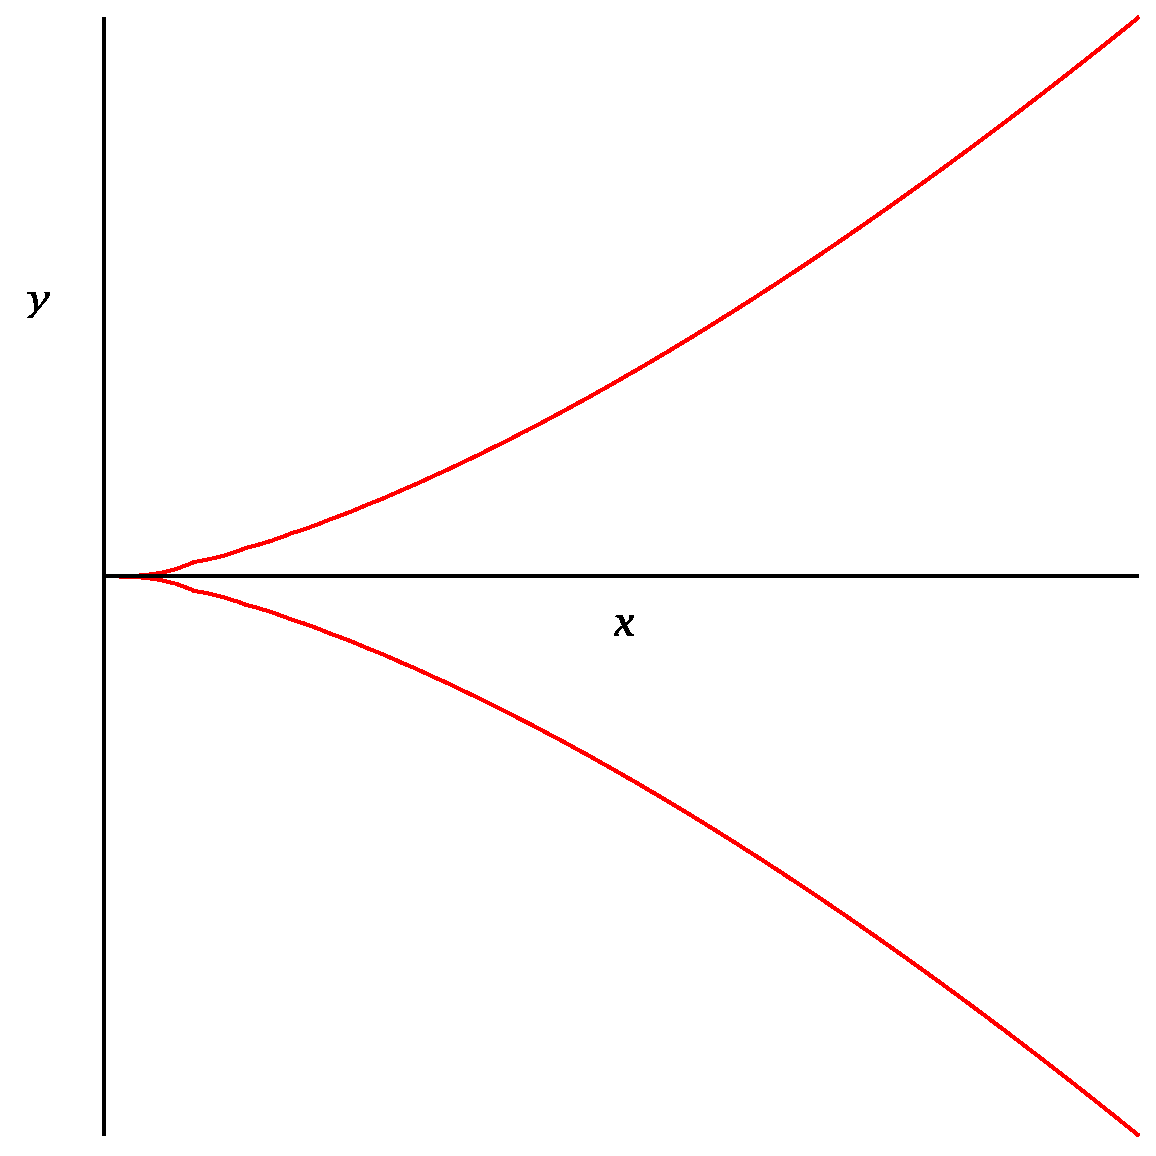
\includegraphics[width=0.45\textwidth]{isogeny/cusp}
  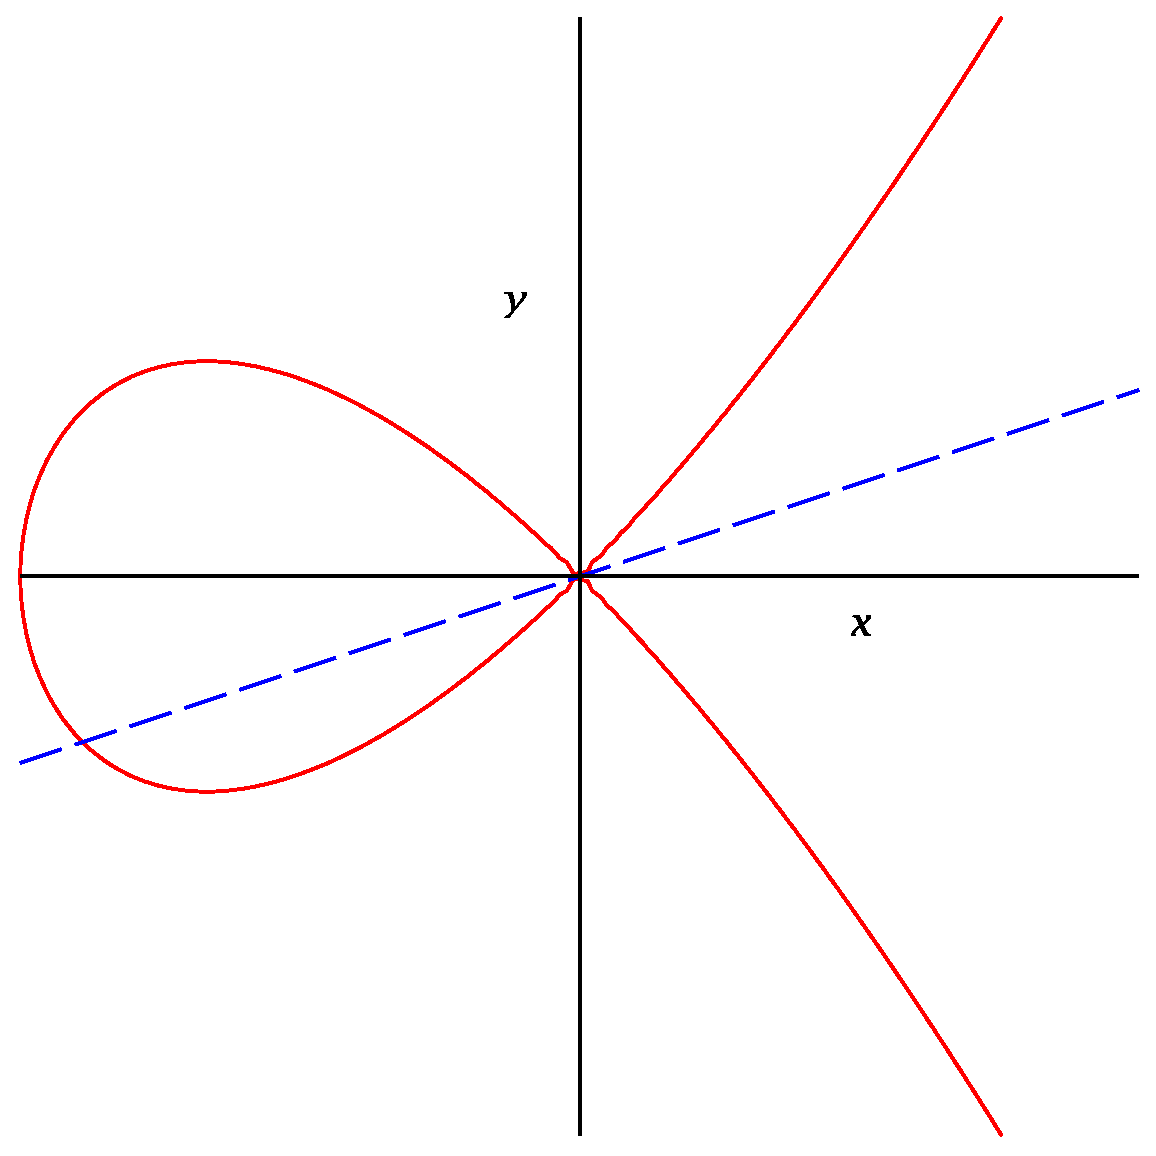
\includegraphics[width=0.45\textwidth]{isogeny/node}
  \caption{Two singular Weierstrass curves. On the left $y^2=x^3$, on
    the right $y^2=x^3+x^2$. On the right we have shown the
    parameterization by the line passing through the origin.}
  \label{fig:singular}
\end{figure}

\begin{definition}[$j$-invariant]
  \index{j-invariant@$j$-invariant}%
  \nomenclature[j]{$j_E$}{$j$-invariant of an elliptic curve $E$}
  We associate to the curve $E$ defined by Eq.~\eqref{eq:112}, the
  $j$-invariant
 \[j_E = \frac{(b_2^2-24b_4)^3}{\Delta_E}\text{.}\]
\end{definition}


\subsection{Group law}
\label{sec:group-law}
Elliptic curves are endowed with a group structure via the
\index{elliptic~curve!group~law}
\index{chord-tangent~law}\emph{chord-tangent law}.

\begin{definition}
  Let $E$ be an elliptic curve and let $P,Q\in\Proj^2$ be two points
  on the curve. Let $L$ be the line passing through $P$ and $Q$, with
  multiplicity two if $P=Q$, and let $R$ be the third intersection
  point with $E$.  Let $L'$ be the line passing through $R$ and
  $\0$. Then the point $P+Q$ is defined as the third point of
  intersection of $L'$ and $E$.
\end{definition}

\begin{figure}[ht]
  \centering
  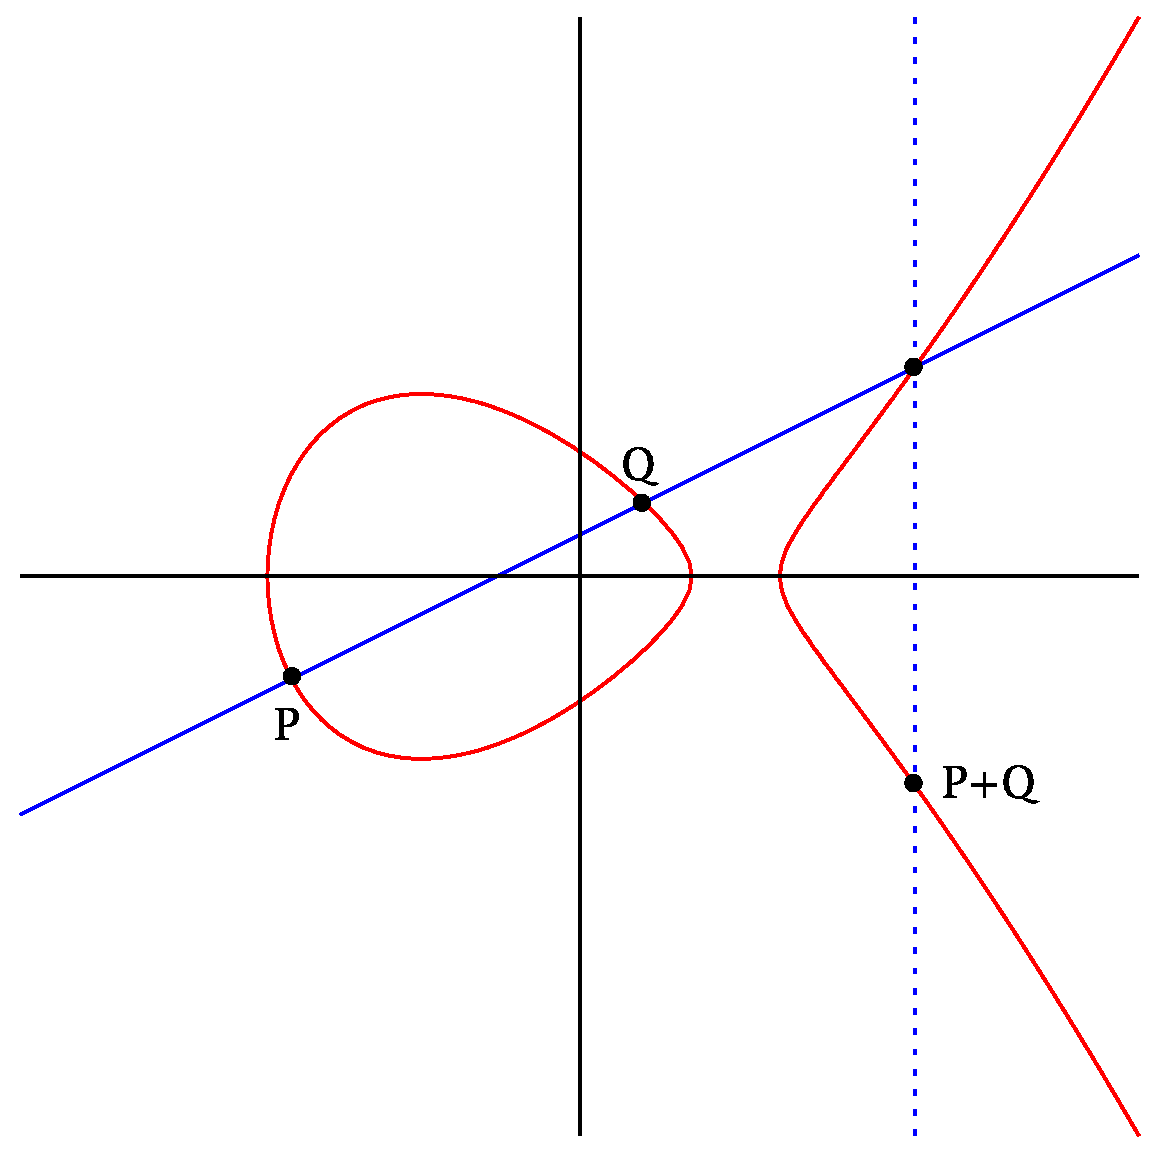
\includegraphics[width=0.5\textwidth]{isogeny/ec-add}
  \caption{Chord-tangent law on an elliptic curve defined over the reals.}
  \label{fig:chord-tangent}
\end{figure}

The definition is pictured in Figure~\ref{fig:chord-tangent}. For a
proof that this defines indeed a group law on the points of $E$, with
$\0$ being the identity element, see \cite[II, $\S2$]{silverman:elliptic}.

\begin{definition}[Rational points]%
  \nomenclature[E]{$E(\K)$}{Set of $\K$-rational points of an elliptic curve $E$}
  Let $E$ be an elliptic curve defined over $\K$, the set of
  \emph{$\K$-rational points}\index{rational~point} $E(\K)$ is 
  \begin{equation}
    \label{eq:119}
    E(\K) = E \cap \Proj^2(\K)
    \text{.}
  \end{equation}
\end{definition}

If $P$ and $Q$ are rational points, the lines $L$ and $L'$ are defined
by equations over $\K$, thus $E(\K)$ forms a subgroup of $E$. To allow
calculations in $E(\K)$ without having to lift the coefficients in an
algebraic closure, it is convenient to give explicit formulas for the
chord-tangent law. 

We shall give the formulas for affine coordinates. From now on, if $P$
is an affine point of $E$, we denote by $x(P)$ its abscissa and by
$y(P)$ its ordinate.

\begin{proposition}
  Let $E$ be the elliptic curve defined by Eq.~\eqref{eq:112}. Let
  $P$, be a point of $E$ different from $\0$, the coordinates of $-P$
  are given by
  \begin{equation}
    \label{eq:120}
    x(-P) = x(P)\text{,}\qquad y(-P)=-y(P) -a_1x(P) - a_3
    \text{.}
  \end{equation}
  Let $P,Q$ be points of $E$ different from $\0$ and let $Q\ne-P$, the
  coordinates of $P+Q$ are given by
  \begin{equation}
    \label{eq:121}
    \begin{aligned}
      \lambda &= \begin{cases}
        \frac{y(Q) - y(P)}{x(Q) -x(P)} &\text{if $P\ne Q$,}\\
        \frac{3x(P)^2+2a_2x(P)+a_4-a_1y(P)}{2y(P)+a_1x(P)+a_3} &\text{if $P=Q$,}
      \end{cases}\\
      x(P+Q) &= \lambda^2+a_1\lambda-a_2-x(P)-x(Q)\text{,}\\
      y(P+Q) &= -(\lambda+a_1)x(P+Q) - y(P) + \lambda x(P)-a_3\text{.}
    \end{aligned}
  \end{equation}
\end{proposition}

\begin{definition}[Kummer surface]
  The \index{Kummer~surface}\emph{Kummer surface} of an elliptic curve
  $E$, denoted by $K_E$\nomenclature[KE]{$K_E$}{Kummer surface of an
    elliptic curve}, is the quotient of $E$ by the equivalence
  relation $P\simeq-P$.
\end{definition}

For $m\in\Z$, we denote by $[m]P$ the point%
\nomenclature[mP]{$[m]P$}{Scalar multiple of a point of an elliptic
  curve} $\overbrace{P+P+\cdots+P}^{m\text{ times}}$ if $m>0$, or the
point $[-m](-P)$ if $m<0$, or $\0$ if $m=0$. 

\begin{remark}
  The Kummer surface can be represented by taking the abscissas of the
  points of $E$. It is not anymore a group, but we can still compute
  scalar multiples of its points. In fact, from the addition formulas
  we deduce for $P\ne-P$
  \begin{equation}
    \label{eq:128}
    x([2]P) = \frac{x^4-b_4x^2-2b_6x-b_8}{4x^3+b_2x^2+2b_4x+b_6}
    \text{,}
  \end{equation}
  where $x=x(P)$; and for $P\ne Q$
  \begin{equation}
    \label{eq:129}
    x(P+Q) + x(P-Q) =
    \frac{2\pi\sigma + b_2\pi + b_4\sigma + b_6}{(x(P)-x(Q))^2}
    \text{,}
  \end{equation}
  where $\pi=x(P)x(Q)$ and $\sigma=x(P)+x(Q)$. 

  Then, to compute $x([n]P)$, we start from $x(P)$ and $x([2]P)$, and
  we iteratively apply
  \begin{equation}
    \label{eq:130}
    \begin{aligned}[]
      [2i]P   &= [2][i]P\text{,}\\
      [2i+1]P &= [i+1]P + [i]P\text{,}
    \end{aligned}
  \end{equation}  
  or
  \begin{equation}
    \label{eq:131}
    \begin{aligned}[]
      [2i+1]P &= [i+1]P + [i]P\text{,}\\
      [2i+2]P &= [2][i+1]P\text{,}
    \end{aligned}
  \end{equation}
  until we reach $[n]P$. This algorithm appeared
  in~\cite{montgomery87} and is sometimes referred to as
  \index{Montgomery's formulas}\emph{Montgomery's formulas}.
\end{remark}

The map
\begin{equation}
  \label{eq:122}
  \begin{aligned}[]
    [m]_E : E(\K) &\ra E(\K)\text{,}\\
    P &\mapsto [m]P
  \end{aligned}
\end{equation}
is a group endomorphisms of $E(\K)$. 

\begin{definition}
  The $m$-th \emph{torsion subgroup} of $E$ is
  \begin{equation}
    \label{eq:123}
    E[m] = \{P\in E(\K) \,|\, [n]P=\0\}
    \text{,}
  \end{equation}
  its points are called%
  \nomenclature[E]{$E[m]$}{$m$-torsion subgroup of an elliptic curve
    $E$}
  \index{elliptic~curve!torsion~subgroup}\index{torsion~point}\emph{$m$-torsion
    points}.
\end{definition}

Since addition is an algebraic map, multiplication by $n$ is algebraic
too. It can be shown that there exist polynomials
$\psi_m,\theta_m,\omega_m\in\K(E)$ such that
\begin{equation}
  \label{eq:124}
  [m](x,y) = \left(\frac{\theta_m(x,y)}{\psi_m(x,y)^2},
    \frac{\omega_m(x,y)}{\psi_m(x,y)^3}\right)
  \text{.}
\end{equation}

\begin{definition}[Division polynomials]
  The polynomial $\psi_m$ is called the
  \index{division~polynomial}\emph{$m$-th division polynomial}.
\end{definition}

\begin{remark}
  The division polynomials can be computed from the addition formulas
  via a double-and-add approach. Their importance comes from the fact
  that $\psi_m$ vanishes on $E[m]$.
\end{remark}

From the formulas for the division polynomials one can deduce the
structure of the $m$-torsion.

\begin{theorem}
  Let $p$ be the characteristic of $\K$. If $p$ does not divide $m$
  \begin{equation}
    \label{eq:126}
    E[m] \isom \Z/m\Z\times\Z/m\Z
    \text{;}
  \end{equation}
  if $p\ne0$, then for every $i>0$ either
  \begin{equation}
    \label{eq:127}
    E[p^i] = \{\0\}\text{,} 
    \qquad\text{or}\qquad E[p^i] \isom \Z/p^i\Z
    \text{.}
  \end{equation}
\end{theorem}

\begin{definition}[Supersingular, ordinary]
  An elliptic curve $E$ is said to be
  \index{elliptic~curve!supersingular}\index{supersingular}\emph{supersingular}
  if $E[p^i]=\{\0\}$ for any $i$; it is said to be
  \index{elliptic~curve!ordinary}\emph{ordinary} otherwise.
\end{definition}

\begin{definition}[Tate module]
  Let $\ell$ be a prime, the \index{Tate~module}\emph{$\ell$-adic Tate
    module}
  $\mathcal{T}_\ell(E)$\nomenclature[Tl]{$\mathcal{T}_\ell(E)$}{$\ell$-adic
    Tate module} is the group
  \begin{equation}
    \label{eq:132}
    \mathcal{T}_\ell(E) = \varprojlim_n E[\ell^n]
  \end{equation}
  with respect to the projections
  \begin{equation}
    \label{eq:133}
    [\ell]_E : E[\ell^{n+1}] \ra E[\ell^{n}]
    \text{.}
  \end{equation}
\end{definition}

\begin{proposition}
  The Tate module has a natural structure of
  $\Z_\ell$-module\nomenclature[Zp]{$\Z_p$}{$p$-adic
    integers\nomnorefpage}. As such
  \begin{equation}
    \label{eq:134}
    \mathcal{T}_\ell(E) \isom
    \begin{cases}
      \Z_\ell\times\Z_\ell &\text{if $\ell\ne p$,}\\
      \Z_p &\text{if $\ell=\car(\K)$ and $E$ is ordinary,}\\
      \{\0\} &\text{if $E$ is supersingular.}
    \end{cases}
  \end{equation}
\end{proposition}


\subsection{Isomorphisms}
\label{sec:isomorphisms}

Let $E$ and $E'$ be two elliptic curves in Weierstrass form over a
field $\K$, they are said to be isomorphic if there is a linear change
of variables that transforms one equation in the other and preserves
the point at infinity.  Then, clearly $E(\clot{\K})$ and
$E'(\clot{\K})$ are isomorphic as groups. If the change of variables
has coefficients in $\K$, the curves are said to be
\index{isomorphism!of~elliptic~curves}\index{elliptic~curve!isomorphic}isomorphic
over $\K$, then $E(\K)$ and $E(\K)$ are isomorphic as groups.

It can be shown that the only such changes of variables are
\begin{equation}
  \label{eq:116}
  \begin{aligned}
    x &= u^2x' + r\text{,}\\
    y &= u^3y' + u^2sx' + t\text{,}
  \end{aligned}
\end{equation}
with $r,s,t,u\in\clot{\K}$.

\begin{proposition}
  Two elliptic curves $E$ and $E'$ in Weierstrass form are isomorphic
  over $\clot{\K}$ if and only if $j_E=j_{E'}$.
\end{proposition}

\index{Weierstrass~form!simplified~form}Weierstrass equations can be
brought via isomorphism to a form that is easier to handle, called
\emph{simplified Weierstrass form}. The following classification is
from~\cite{connell:elliptic}.

\begin{proposition}[Simplified Weierstrass form]
  Any elliptic curve is isomorphic to one of the following Weierstrass
  forms:
  \begin{itemize}
  \item If $\car(\K)=0$ or $\car(\K)>3$
    \begin{equation}
      \label{eq:weierstrass>3}
      E\;:\;y^2 = x^3 + ax + b 
      \qquad\text{and}\qquad
      j_E = \frac{1728(4a)^3}{16(4a^3 + 27b^2)}
      \text{;}
    \end{equation}
  \item if $\car(\K)=3$ and $E$ is ordinary
    \begin{equation}
      \label{eq:weierstrass=3}
      E\;:\;y^2 = x^3 + ax^2 + b
      \qquad\text{and}\qquad
      j_E = -\frac{a^3}{b}
      \text{;}
    \end{equation}
  \item if $\car(\K)=3$ and $E$ is supersingular
    \begin{equation}
      \label{eq:136}
      E\;:\;y^2=x^3 + ax+b
      \qquad\text{and}\qquad
      j_E=0
      \text{;}
    \end{equation}
  \item if $\car(\K)=2$ and $E$ is ordinary
    \begin{equation}
      \label{eq:weierstrass=2}
      y^2 + xy = x^3 + ax^2 + b
      \qquad\text{and}\qquad
      j_E = \frac{1}{b}
      \text{;}
    \end{equation}
  \item if $\car(\K)=2$ and $E$ is supersingular
    \begin{equation}
      \label{eq:137}
      E\;:\; y^2 + a_3y = x^3 + a_4x + a_6
      \qquad\text{and}\qquad
      j_E = 0
      \text{.}
    \end{equation}
  \end{itemize}
\end{proposition}

\begin{definition}[Twist]
  Two non-isomorphic elliptic curves $E$ and $E'$ over $\K$ such that
  $j_E=j_{E'}$ are called \index{twist}\emph{twists}.
\end{definition}

A twist is isomorphic over the algebraic closure $\clot{\K}$. The
\index{twist!degree~of~a}degree of the twist is the degree of the
smallest extension $\K'/\K$ such that the twist is isomorphic over
$\K$.

\begin{proposition}
  Any curve has a quadratic twist. Any twist of ordinary elliptic
  curves is quadratic.
\end{proposition}


\subsection{Isogenies}
\label{sec:isogenies}

\begin{definition}[Isogeny]
  Let $E$ and $E'$ be elliptic curves, an
  \index{isogeny}\emph{isogeny} $E\ra E$ is a morphism of varieties
  that preserves the point at infinity.
\end{definition}

It turns out that isogenies preserve the group structure.

\begin{theorem}
  Let $\I:E\ra E'$ be an isogeny, then it is a group morphism
  $E(\clot{\K})\ra E'(\clot{\K})$. It is surjective and its kernel is
  finite. Furthermore, if $\I$ is defined over $\K$, then its
  restriction to $E(\K)$ is a group morphism $E(\K)\ra E'(\K)$.
\end{theorem}

\begin{definition}[Degree]
  Let $\I$ be an isogeny and
  \index{degree!of~an~isogeny}\index{isogeny!degree}define
  \begin{equation}
    \label{eq:138}
    \begin{aligned}
      \dual{\I}:\clot{K}(E')&\ra\clot{K}(E)\\
      f &\ra f\circ\I
      \text{.}
    \end{aligned}
  \end{equation}
  The \emph{separable (resp. inseparable) degree} of $\I$, denoted by
  $\deg_s\I$ (resp. $\deg_i\I$), is the separable (resp. inseparable)
  degree of the field extension $\clot{\K}(E)/\I(\clot{\K}(E'))$. The
  \emph{degree} of $\I$ is $\deg\I=\deg_s\I\deg_i\I$.

  An isogeny is called \index{isogeny!separable}\emph{separable} if
  $\deg_i\I=1$, \index{isogeny!inseparable}\emph{inseparable}
  otherwise. It is called
  \index{isogeny!purely~inseparable}\emph{purely inseparable} if
  $\deg_s=1$.
\end{definition}

\begin{theorem}
  Let $\I$ be an isogeny, its kernel contains $\deg_s\I$ elements.
\end{theorem}

One example of isogeny is the map $[m]$, it is a separable isogeny of
degree $m^2$. If $\K$ has characteristic $p$, then the map
\begin{equation}
  \label{eq:139}
  \frobisog : (x,y) \mapsto (x^p,y^p)
\end{equation}
is a purely inseparable isogeny of degree $p$, called the
\index{Frobenius~isogeny}\emph{Frobenius
  isogeny}\nomenclature[f]{$\frobisog$}{Frobenius isogeny:
  $(x,y)\mapsto(x^p,y^p)$}. If $\K$ is a perfect field, any purely
inseparable isogeny is a power of $\frobisog$.

\begin{theorem}
  Any isogeny can be factored in a product of a separable and a purely
  inseparable isogeny.
\end{theorem}

One important property about isogenies is that they factor the
multiplication by $m$ map.

\begin{definition}[Dual isogeny]
  Let $\I : E \rightarrow E'$ be a degree $m$ isogeny. There exists an
  unique isogeny $\hat{\I} : E' \rightarrow E$, called the
  \index{dual~isogeny}\index{isogeny!dual}\emph{dual isogeny} such
  that
  \[\I\circ\hat{\I} = [m]_E \qquad\text{and}\qquad \hat{\I}\circ\I =
  [m]_{E'}\]
\end{definition}

By endomorphism we mean an isogeny $E\ra E$. The multiplication maps
are endomorphisms, thus $\End(E)$ contains a copy of $\Z$.  The main
theorem about the endomorphism ring $\End(E)$ is the following.

\begin{theorem}
  The endomorphism ring is either isomorphic to $\Z$, or to an order
  in a quadratic imaginary field, or to an order in a quaternion
  algebra.
\end{theorem}

If $\car(\K)\ne0$, we can exclude the case $\Z$, because $\End(E)$
contains the Frobenius isogeny. Furthermore, in the two cases
\begin{itemize}
\item $\car(\K)=0$,
\item $\K$ perfect and $E$ ordinary
\end{itemize}
$\End(E)$ cannot be an order in a quaternion algebra, thus it is
commutative.


\section{Curves over $\C$}
\label{sec:curves-over-c}
Elliptic curves defined over $\C$ have a very simple structure.

\begin{definition}[Lattice]
  A \index{lattice}\emph{lattice} $\Lambda\subset\C$ is a discrete
  additive subgroup of $\C$ that contains a basis of the $\R$-vector
  space $\C$. Two lattices $\Lambda_1,\Lambda_2$ are said to be
  \emph{homothetic} if $\Lambda_1=\alpha\Lambda_2$ for some
  $\alpha\in\C^{\ast}$.
\end{definition}

\begin{definition}[Elliptic function]
  Let $\Lambda$ be a lattice. An
  \index{elliptic~function}\emph{elliptic function} on $\Lambda$ is a
  meromorphic function $f$ on $\C$ such that
  \begin{equation}
    \label{eq:141}
    f(z+\omega) = f(z)
  \end{equation}
  for any $\omega\in\Lambda$.  The set of elliptic functions on
  $\Lambda$ is denoted by $\C(\Lambda)$.
\end{definition}

An example of elliptic function is the
\index{Weierstrass~function@Weierstrass~$\wp$-function}\emph{Weierstrass
  $\wp$-function}\nomenclature[p]{$\wp$}{Weierstrass $\wp$-function}
\begin{equation}
  \label{eq:142}
  \wp(z;\Lambda) = \frac{1}{z^2} + \sum_{\omega\in\Lambda\backslash\{0\}}\frac{1}{(z-\omega)^2}-\frac{1}{\omega^2}
  \text{,}
\end{equation}
\begin{theorem}
  Let $\Lambda$ be a lattice, then $\C(\Lambda) = \C(\wp(z),\wp'(z))$.
\end{theorem}

For $k>1$, we define the \index{Eisenstein~series}\emph{Eisenstein
  series} $G_{2k}$\nomenclature[G2k]{$G_{2k}$}{Eisenstein series} as
\begin{equation}
  \label{eq:143}
  G_{2k}(\Lambda) = \sum_{\omega\in\Lambda\backslash\{0\}}\frac{1}{\omega^2}
  \text{.}
\end{equation}

\begin{theorem}
  The Laurent series expansion of $\wp(z)$ at $0$ is
  \begin{equation}
    \label{eq:144}
    \wp(z) = \frac{1}{z^2} + \sum_{k=1}^\infty (2k+1)G_{2k+2}z^{2k}
    \text{.}
  \end{equation}
  At any $z\not\in\Lambda$, the function $\wp(z)$ satisfies the
  differential equation
  \begin{equation}
    \label{eq:145}
    {\wp'}^2 = 4\wp - 60G_4\wp - 140G_6
    \text{.}
  \end{equation}
\end{theorem}

We set $g_2(\Lambda)=60G_4(\Lambda)$ and $g_3(\Lambda)=140G_6(\Lambda)$.

\begin{theorem}
  Let $E$ be the curve 
  \begin{equation}
    \label{eq:146}
    E\;:\: y^2=4x^3-g_2(\Lambda)x-g_3(\Lambda)
    \text{.}
  \end{equation}
  The map
  \begin{equation}
    \label{eq:147}
    \begin{aligned}
      \phi: \C/\Lambda &\ra E(\C)\\
      z &\mapsto
      \begin{cases}
        \0 &\text{if $z=0$,}\\
        (\wp(z), \wp'(z)) &\text{otherwise,}
      \end{cases}
    \end{aligned}
  \end{equation}
  is an isomorphism of Riemann surfaces and a group homomorphism. 
\end{theorem}

If $\Lambda$ is a lattice, we denote by $E_\Lambda$ the elliptic curve
corresponding to it as in Eq.~\eqref{eq:146}.

\begin{theorem}
  Let $\Lambda_1,\Lambda_2$ be lattices and let $a\in\C^\ast$ such that
  $a\Lambda_1\subset\Lambda_2$. The map
  \begin{equation}
    \label{eq:148}
    \begin{aligned}
      \phi_a:\C/\Lambda_1&\ra\C/\Lambda_2\\
      z&\mapsto az
    \end{aligned}
  \end{equation}
  is holomorphic. The map $E_{\Lambda_1}\ra E_{\Lambda_2}$ induced by
  $\phi_a$ is an isogeny.
\end{theorem}

The correspondences we just defined are actually equivalences.

\begin{theorem}
  The category of elliptic curves with isogenies as maps is equivalent
  to the category of lattices up to homothety with maps $z\mapsto az$
  such that $a\Lambda_1\subset\Lambda_2$.
\end{theorem}

Thus to any elliptic curve there is an unique lattice $\Lambda$
associated up to homothety; the addition law on $\C/\Lambda$ is just
addition in $\C$, and an isogeny can be obtained by an $a\in\C$ such
that $a\Lambda_1\subset\Lambda_2$.



\section{Curves over finite fields}
\label{sec:curves-over-finite}
We saw previously that an elliptic curve defined over a field of
characteristic $p\ne0$ has an isogeny
\begin{equation}
  \label{eq:150}
  \frobisog:(x,y)\mapsto(x^p,y^p)
\end{equation}
called Frobenius isogeny. If the curve $E$ is defined over the field
$\F_q$ with $q=p^d$, then $d$ iterations of the Frobenius map give the
isogeny
\begin{equation}
  \label{eq:151}
  \frobisog_q\eqdef\frobisog^d:(x,y)\mapsto(x^q,y^q)
  \text{.}
\end{equation}

The map $\frobisog_q$ is an endomorphism of $E$ and fixes the points
of $E(\F_q)$; it is called the \index{Frobenius
  endomorphism}\emph{Frobenius endomorphism} of $E$. It plays an
important role in determining the cardinality of $E(\F_q)$.

\begin{theorem}[Hasse]
  \index{Hasse~bound}
  The minimal polynomial of $\frobisog_q$ in $\End(E)$ is of the form
  \begin{equation}
    \label{eq:152}
    \frobisog_q^2 - c\frobisog_q + q = 0
  \end{equation}
  with $\lvert c\rvert\le2\sqrt{q}$.
\end{theorem}

Since $\frob_q$ acts as the identity on $E(\F_q)$, this implies
\begin{equation}
  \label{eq:153}
  \card{E(\F_q)} = q+1-c
  \qquad\text{with } \lvert c\rvert\le2\sqrt{q}
  \text{.}
\end{equation}

\begin{theorem}
  Two elliptic curves $E,E'$ defined over $\F_q$ are isogenous if and
  only if $\card{E(\F_q)}=\card{E(\F_q)}$.
\end{theorem}


\section{Vélu formulas}
\label{sec:velu-formulas}
For any finite subgroup $G \subset E(\clot{\K})$, Vélu formulas
\cite{Vel71} give in a canonical way an elliptic curve $\bar{E}$ and
an explicit isogeny $\I:E\rightarrow \bar{E}$ such that
$\ker\I=G$. The isogeny is $\K$-rational if and only if the polynomial
vanishing on the abscissae of $G$ belongs to $\K[X]$.

In practice, if $E$ is defined over $\F_q$ and if
\[h(X) = \prod_{\substack{P\in G\\P\ne\0}}(X - x(P)) \in \F_q[X]\]
is known, Vélu formulas compute a rational function
\begin{equation}
  \label{eq:isog}
  \bar{\I}(x,y) = \left(\frac{g(x)}{h(x)}, \frac{k(x,y)}{l(x)}\right)  
\end{equation}
and a curve $\bar{E}$ such that $\bar{\I} : E\rightarrow\bar{E}$ is an
$\F_q$-rational isogeny of kernel $G$. A consequence of Vélu formulas
is
\begin{equation}
  \label{eq:velu-deg}
  \deg g = \deg h + 1 = \card{G}
  \text{.}
\end{equation}

Given two curves $E$ and $E'$, Vélu formulas reduce the problem of
finding an explicit isogeny between $E$ and $E'$ to that of finding
the kernel of an isogeny between them. Once the polynomial $h(X)$
vanishing on $\ker\I$ is found, the explicit isogeny is computed
composing Vélu formulas with the isomorphism between $\bar{E}$ and
$E'$ as in figure \ref{fig:velu}.

\begin{figure}
  \centering
  \[\xymatrix{
    E \ar[r]^{\bar{\I}} \ar[rd]^\I & \bar{E} \ar[d]^{\simeq}\\
    & E'
  }\]
  \caption{Using Vélu formulas to compute an explicit isogeny.}
  \label{fig:velu}
\end{figure}





% Local Variables:
% mode:flyspell
% ispell-local-dictionary:"american"
% mode:TeX-PDF
% mode:reftex
% TeX-master: "../these"
% End:
%
% LocalWords:  Schreier Artin pseudotrace frobenius bivariate Joux Sirvent FFT
% LocalWords:  Couveignes isogenies Schoof isogeny cryptosystems Lercier
% LocalWords:  precomputation arithmetics polylogarithmic Karatsuba
% LocalWords:  endomorphisms


\chapter{Algorithms in large characteristic}
\section{Atkin}
\section{Elkies}
\section{BMSS}

\chapter{Algorithms in small characteristic}
\label{cha:algor-small-char}
\section{Couveignes first algorithm}
\section{Lercier}
\section{Lercier-Sirvent}
%% these.tex
%% Copyright 2010 Luca De Feo
%% All rights reserved


\section{Couveignes' algorithm}
\label{sec:C2}

In this section we describe Couveignes' algorithm to compute isogenies
between ordinary elliptic curves in arbitrary characteristic, as it
was originally presented in~\cite{couveignes96}. In the next sections
we will discuss more efficient variants of this algorithm; to
distinguish between the variants, we call \ctwo{} this original
version (it is to be understood that \alg{C1} would be the code-name
of the other algorithm by Couveignes, appeared in~\cite{couveignes94},
that we will not present in this document).

\ctwo{} takes as input two elliptic curves $E, E'$ and an integer
$\ell$ prime to $p$, and it returns, if it exists, an $\F_q$-rational
isogeny of degree $\ell$ between $E$ and $E'$. It only works in odd
characteristic.

\subsection{The original algorithm}
Suppose there exists an $\F_q$-rational isogeny
$\I:E\rightarrow E'$ of degree $\ell$. Since $\ell$ is prime to $p$
one has $\I(E[p^k]) = E'[p^k]$ for any $k$.

Recall that $E[p^k]$ and $E'[p^k]$ are cyclic groups. \ctwo{} iteratively
computes generators $P_k,P_k'$ of $E[p^k]$ and $E'[p^k]$
respectively. Now \ctwo{} makes the guess $\I(P_k) = P_k'$; then, if $\I$
is given by rational fractions as in~\eqref{eq:159},
\begin{equation}
  \label{eq:C2:I}
  \frac{g\bigl(x([i]P_k)\bigr)}{h\bigl(x([i]P_k)\bigr)} = x([i]P_k')
  \quad\text{for $i\in\Z/p^k\Z$,} 
\end{equation}
and \titleref{sec:velu-formulas} imply that
\begin{equation}
  \label{eq:velu-deg}
  \deg g = \deg h + 1 = \ell
  \text{.}
\end{equation}


Using \eqref{eq:C2:I} one can compute the rational fraction
$\frac{g(X)}{h(X)}$ through \hyperref[sec:eucl-algor-rati]{Cauchy
  interpolation} over the points of $E[p^k]$ for $k$ large enough. \ctwo{}
takes $p^k \ge 4\ell +1$, interpolates the rational fraction and then
checks that it corresponds to the restriction of an isogeny to the
$x$-axis. If this is the case, the whole isogeny is computed through
Vélu formulas and the algorithm terminates. Otherwise the guess
$\I(P_k) = P_k'$ was wrong, then \ctwo{} computes a new generator for
$E'[p^k]$ and starts over again.

We now go through the details of the algorithm.

\paragraph{The $p$-torsion}
The computation of the $p$-torsion points follows from the work of
Gunji~\cite{gunji76}. Here we suppose $p\ne2$.

\begin{definition}
  \label{def:hasse}
  Let $E$ have equation $y^2 = f(x)$. The \emph{Hasse invariant} of
  $E$, denoted by $H_E$, is the coefficient of $X^{p-1}$ in
  $f(X)^{\frac{p-1}{2}}$.
\end{definition}

Gunji shows the following proposition.

\begin{proposition}
  \label{th:gunji}
  Let $c_1,\ldots,c_{p-1}$ be the roots of $X^{p-1}-H_E$ in its
  splitting field. The abscissas of the abscissas of the $p$-torsion
  points of $E$ are given by
  \[X_i^p = \frac{\Delta_0^2 - a_6c_i^2\Delta_1^2}{4c_i^2}\text{,}\]
  where $\Delta_0$ and $\Delta_1$ are the following determinants
  \begin{equation}
    \begin{gathered}
      \Delta_0 = \begin{vmatrix}
        \beta_1 & \alpha_2 & 0 & 0 & \ldots & 0\\
        \delta_1 & \gamma_2 - c^2 & \beta_3 & \alpha_4 & \ddots & \vdots \\
        0 & \delta_2 & \gamma_3 - c^2 & \beta_4 & \ddots & 0 \\
        \vdots & \ddots & \delta_3 & \ddots & \ddots & \alpha_r \\
        \vdots & & \ddots & \ddots & \ddots & \beta_r \\
        0 & \ldots & \ldots & 0 & \delta_{r-1} & \gamma_r - c^2
      \end{vmatrix}\text{,}\\
      \Delta_1 = \begin{vmatrix}
        \gamma_2 - c^2 & \beta_3 & \alpha_4 & \ldots & 0 \\
        \delta_2 & \gamma_3 - c^2 & \beta_4 & \ddots & \vdots \\
        0 & \delta_3 & \ddots & \ddots & \alpha_r \\
        \vdots & \ddots & \ddots & \ddots & \beta_r \\
        0 & \ldots & 0 & \delta_{r-1} & \gamma_r - c^2
      \end{vmatrix}\text{,}
    \end{gathered}
  \end{equation}
  with $r = \frac{p-1}{2}$, $\alpha_\nu = \nu(\nu-1)a_6$, $\beta_\nu =
  \nu(\nu-\frac{1}{2})a_4$, $\gamma_\nu = \nu^2a_2$ and $\delta_\nu =
  \nu(\nu+\frac{1}{2})$ ($\Delta_1$ is set to $1$ when $r = 1$).
\end{proposition}

In what follows we let $c$ be any $(p-1)$-th root of $H_E$. Then
Gunji's formulas imply that the $p$-torsion points are defined in
$\F_q[c]$ and their abscissas are defined in $\F_q[c^2]$.


\paragraph{The $p^k$-torsion}
$p^k$-torsion points are iteratively computed via $p$-descent. The
basic idea is to split the multiplication map as $[p] = \frobisog\circ
V$ and invert each of the components. The purely inseparable isogeny
$\frobisog$ is just a Frobenius map and the separable isogeny $V$ can
be computed by \hyperref[sec:velu-formulas]{Vélu formulas} once the
$p$-torsion points are known. Although this is reasonably efficient,
pulling $V$ back may involve factoring polynomials of degree $p$ in
some extension field.

A finer way to do the $p$-descent, as suggested in the original
paper~\cite{couveignes96}, is to use the work of
Voloch~\cite{voloch90}. Suppose $p\ne2$, let $E$ and $\widetilde{E}$
have equations respectively
\begin{align*}
  y^2&=f(x)=x^3+a_2x^2+a_4x+a_6 \;\text{,}\\
  \tilde{y}^2&=\tilde{f}(\tilde{x}) = \tilde{x}^3 +
  \sqrt[p]{a_2}\tilde{x}^2 + \sqrt[p]{a_4}\tilde{x} + \sqrt[p]{a_6}
  \;\text{,}
\end{align*}
set
 \begin{equation}
  \label{eq:voloch:cover}
  \tilde{f}(X)^{\frac{p-1}{2}} = \alpha(X) + H_{\widetilde{E}}X^{p-1} + X^p\beta(X)
\end{equation}
with $\deg \alpha < p-1$ and $H_{\widetilde{E}}$ the Hasse invariant
of $\widetilde{E}$. Voloch shows the following proposition.

\begin{proposition}
  \label{th:voloch}
  Let $\tilde{c} = \sqrt[p-1]{H_{\widetilde{E}}}$, the cover of
  $\widetilde{E}$ defined by
  \begin{equation}
    \label{th:voloch:cover}
    C:\; \tilde{z}^p - \tilde{z} = \frac{\tilde{y}\beta(\tilde{x})}{\tilde{c}^p}
  \end{equation}
  \pdfmcone{The "étale" property is from the original
    statement in Voloch's paper, I guess it is necessary to guarantee
    that the cover is a group morphism.  Not that I really understand
    what it means exactly, but is this a reason to change the
    statement?} is an étale cover of degree $p$ and is isomorphic to
  $E$ over $\F_q[\tilde{c}]$; the isomorphism is given by
  \begin{equation}
    \label{th:voloch:isom}
    \left\{
      \begin{aligned}
        (\tilde{x}, \tilde{y}) &= V(x, y)\\
        \tilde{z} &= -\frac{y}{\tilde{c}^p}\sum_{i=1}^{p-1}\frac{1}{x - x([i]P_1)}
      \end{aligned}
    \right.
  \end{equation}
  where $P_1$ is a primitive $p$-torsion point of $E$.
\end{proposition}

The descent is then performed as follows: starting from a point $P$ on
$E$, first pull it back along $\frobisog$, then take one of its
pre-images in $C$ by solving equation \eqref{th:voloch:cover}, finally
use equation \eqref{th:voloch:isom} to land on a point $P'$ in $E$.
The proposition guarantees that $[p]P' = P$. The descent is pictured
in figure \ref{fig:voloch}.

\begin{figure}
  \centering
  \[
  \xymatrix{\widetilde{E}\ar@/^/[r]^{\frobisog} & E\ar@/^/[l]^{V}}
  %%
  \qquad
  %%
  \xymatrix{
    \widetilde{E}\ar@/^/[r]^{\frobisog} & E\ar@/^/@{-->}[l]^{V}\ar[d]_{\simeq}\\
    & C\ar@/^/[ul]
  }
  \]
  
  \caption{Two ways of doing the $p$-descent: standard on the left and via a degree $p$ cover on the right}
  \label{fig:voloch}
\end{figure}


The reason why this is more efficient than a standard descent is the
shape of equation \eqref{th:voloch:cover}: it is an Artin-Schreier
equation and it can be solved by the techniques of
Chapter~\ref{cha:artin-schr-towers} (or by linear algebra, as was
suggested in~\cite{couveignes96}). Once a solution $\tilde{z}$ to
\eqref{th:voloch:cover} is known, solving in $x$ and $y$ the bivariate
polynomial system \eqref{th:voloch:isom} takes just a GCD computation
(explicit formulas were given by Lercier
in~\cite[$\S$6.2]{lercier-algorithmique}, we give some slightly
improved ones in Section \ref{sec:implementation}). Compare this with
a generic factoring algorithm needed by standard descent.

In this section we assume that the Artin-Schreier equations are solved
using linear algebra. The impact of
Chapter~\ref{cha:artin-schr-towers} over Couveignes' algorithm is
discussed in the next section.


\paragraph{Cauchy interpolation}
Interpolation reconstructs a polynomial from the values it takes on
some points; Cauchy interpolation reconstructs a rational fraction. As
we saw in Section~\ref{sec:eucl-algor-rati}, the Cauchy interpolation
algorithm is divided in two phases: first find the polynomial $P$
interpolating the evaluation points, then use the Euclidean algorithm
to find a rational fraction congruent to $P$ modulo the polynomial
vanishing on the points.

Cauchy interpolation needs $n+1$ points to reconstruct a degree
$(k,n-k)$ rational fraction. This, together with \eqref{eq:velu-deg},
justifies the choice of $k$ such that $p^k \ge 4\ell+1$. Some of our
variants of \ctwo{} will interpolate only on the primitive $p^k$-torsion
points, thus requiring the slightly larger bound $\euler(p^k) \ge
4\ell+1$. This is not very important to our asymptotical analysis
since in both cases $p^k \in O(\ell)$.

\paragraph{Recognising the isogeny}
Once the rational fraction $\frac{g(X)}{h(X)}$ has been computed, one
has to verify that it is indeed an isogeny. The first test is to check
that the degrees of $g$ and $h$ match equation \eqref{eq:velu-deg}: if
this is not the case, the equation can be discarded right away and the
algorithm can go on with the next trial. Next, one can check that $h$
is indeed the square of a polynomial (or, if $\ell$ is even, the
product of one factor of the $2$-division polynomial and a square
polynomial). These two tests are usually enough to detect an
isogeny. In case a higher confidence is needed, one can evaluate the
rational fraction on some random points of $E$ and check that it is
indeed a group morphism. Finally, if a deterministic proof is needed,
one can compute the $\ell$-division polynomial modulo $h$ and verify
that it is equal to $0$.


\subsection{The case \texorpdfstring{$p=2$}{p=2}}
\label{sec:p=2}
The algorithm, as we presented it, only works when $p\ne2$, it is
however an easy matter to generalise it. The only phase that does not
work is the computation of the $p^k$-torsion points. For curves in the
simplified Weierstrass form \eqref{eq:weierstrass=2} the only
$2$-torsion point is $(0,\sqrt{b})$.

\pdfmcone{"Kummer surface" -> "Kummer variety".}
Voloch formulas are hard to adapt, nevertheless a $2$-descent on the
\hyperref[def:kummer]{Kummer variety} of $E$ can easily be performed
since the doubling formula reads
\begin{equation}
  x([2]P) = \frac{b}{x(P)^2} + x(P)^2 =
  \frobisog\left(\frac{\sqrt{b} + x(P)^2}{x(P)} \right) = \frobisog\circ V
  \;\text{.}
\end{equation}
Given point $x_P$ on $K_E$, a pull-back along $\frobisog$ gives a
point $\tilde{x}_P$ on $K_{\widetilde{E}}$. Then pulling $V$ back
amounts to solve
\begin{equation}
  \label{eq:2-descent}
  x^2 + \tilde{x}_Px = \sqrt{b}
\end{equation}
and this can be turned in an Artin-Schreier equation through the
change of variables $x \rightarrow x'\tilde{x}_P$.

\pdfmctwo{y coordinates are not needed
  in the second phase, but they are so badly needed in the descent
  using Voloch formulas. Thus the case p=2 is the only one where we can
  ignore the y coordinate.} From the descent on the Kummer varieties
one could deduce a full $2$-descent on the curves by solving a
quadratic equation at each step in order recover the $y$ coordinate,
but this would be too expensive. Fortunately, the $y$ coordinates are
not needed by the subsequent steps of the algorithm, thus one may
simply ignore them. Observe in fact that even if $K_E$ does not have a
group law, the restriction of scalar multiplication is well defined
and can be computed through Montgomery formulas as described in
Remark~\ref{rk:montgomery}. This is enough to compute all the
abscissas of the points in $E[p^k]$ once a generator is known.


\subsection{Complexity analysis}
\label{sec:C2:complexity}
Analyzing the complexity of \ctwo{} is a delicate matter since the
algorithm relies on some black-box computer algebra algorithms in
order to deal with finite extensions of $\F_q$. The choice of the
actual algorithms may strongly influence the overall complexity of \ctwo{}.
In this section we will only give some lower bounds on the complexity
of \ctwo{}, since a much more accurate complexity analysis will be carried
out in Section \ref{sec:C2-AS}.

\paragraph{$p$-Torsion}
Applying Gunji formulas first requires to find $c$ and $c'$, $(p-1)$-th
roots of $H_E$ and $H_{E'}$, and build the field extension $\F_q[c] =
\F_q[c']$. Independently of the actual algorithm used, observe that in
the worst case $\F_q[c]$ is a degree $p-1$ extension of $\F_q$, thus
simply representing one of its elements requires $\Theta(pd)$ elements
of $\F_p$.

Subsequently, the main cost in Gunji's formulas is the computation of
the determinant of a $\frac{p-1}{2}\times\frac{p-1}{2}$
quadri-diagonal matrix (see~\cite{gunji76}). This takes $\Theta(p^2)$
operations in $\F_q[c]$ by Gauss elimination, that is no less than
$\Omega(p^3d)$ operations in $\F_p$.

\paragraph{$p^k$-Torsion}
During the $p$-descent, factoring of equations \eqref{th:voloch:cover}
or \eqref{eq:2-descent} may introduce some field extensions over
$\F_q[c]$. Recall that an Artin-Schreier polynomial is either
irreducible or totally split (see
Proposition~\ref{th:artin-schreier}), so at each step of the
$p$-descent we either stay in the same field or we take a degree $p$
extension. This shows that in the worst case we have to take an
extension of degree $p^{k-1}$ over $F_q[c]$. The following
proposition, which is a generalization
of~\cite[Proposition~26]{lercier-algorithmique}, states precisely how
likely this case is.

\begin{proposition}
  \label{th:tower}
  Let $E$ be an elliptic curve over $\F_q$, we denote by $\U_i$ the
  smallest field extension of $\F_q$ such that $E[p^i]\subset
  E(\U_i)$. For any $i\ge1$, either $[\U_{i+1}:\U_i] = p$ or
  $\U_{i+1}=\U_i=\cdots=\U_1$.
\end{proposition}

Before proving the proposition, we shall state a lemma. Its proof is
elementary and can be found in~\cite[$\S6.1$]{lercier-algorithmique}.

\begin{lemma}
  \label{th:lercier-p-adic}
  Let $p$ be a prime and let $c$ be prime to $p$. For any $k>1$, let
  $\ord_k(c)$ be the order of $c$ in $\Z/p^k\Z$. Then
  $\ord_{k+1}(c)=\ord_k(c)$ implies $\ord_k(c)=\ord_{k-1}(c)$.
\end{lemma}

\begin{proof}[Proof of Propositon~\ref{th:tower}]
  Observe that the action of the Frobenius $\frobisog$ on $E[p]$ is
  just multiplication by the trace $t$, in fact the equation
  \[\frobisog^2 - [t \bmod p]\circ\frobisog + [q \bmod p] = 0\]
  has two solutions, namely $[t \bmod p]$ and $[0 \bmod p]$, but the
  second can be discarded since it would imply that $\frobisog$ has
  non-trivial kernel.  By lifting this solution, one sees that the
  action of $\frobisog$ on the Tate module $\mathcal{T}_p(E)$ is equal
  to multiplication by some $\tau\in\Z_p$.

  Let $G$ be the absolute Galois group of $\F_q$, there is a well
  known action of $G$ on $\mathcal{T}_p(E)$. Since $G$ is generated by
  the Frobenius automorphism of $\F_q$, the restriction of this action
  to $E[p^k]$ is equal to the action (via multiplication) of the
  subgroup of $(\Z/p^k\Z)^\ast$ generated by $\tau_k = \tau \bmod
  p^k$. Hence $[\U_k:\F_q] = \ord(\tau_k)$.

  Then, for any $k>1$, Lemma~\ref{th:lercier-p-adic} applied to
  $\tau_{k+1}=\tau\bmod p^{k+1}$ shows that
  $\ord(\tau_{k+1})=\ord(\tau_k)$ implies
  $\ord(\tau_k)=\ord(\tau_{k-1})$ and this concludes the proof.
\end{proof}


Thus for any elliptic curve there is an $i_0$ such that $[\U_i:\U_1] =
p^{i-i_0}$ for any $i \ge i_0$. This shows that the worst and the
average case coincide since for any fixed curve $[\U_k:\U_1] \in
\Theta(p^k)$ asymptotically. In this situation, one needs
$\Theta(p^kd)$ elements of $\F_p$ to store an element of $\U_k$.

Now the last iteration of the $p$-descent needs to solve an
Artin-Schreier equation in $\U_k$. To do this \ctwo{} precomputes the
matrix of the $\F_q$-linear application $(x^q-x):\U_k\rightarrow\U_k$
and its inverse, plus the matrix of the $\F_p$-linear application
$(x^p-x):\F_q\rightarrow\F_q$ and its inverse. The former is the most
expensive one and takes $\Theta(p^{\omega k})$ operations in $\F_q$,
that is $\Omega(p^{\omega k}d) = \Omega(\ell^\omega d)$ operations in
$\F_p$, plus a storage of $\Theta(\ell^2d)$ elements of
$\F_p$. Observe that this precomputation may be used to compute any
other isogeny with domain $E$.

After the precomputation has been done, \ctwo{} successively applies
the two inverse matrices; details can be found
in~\cite[$\S$2.4]{couveignes96}. This costs at least
$\Omega(\ell^2d)$.


\paragraph{Interpolation}
The most expensive part of Cauchy interpolation is the polynomial
interpolation phase. In fact, simply representing a polynomial of
degree $p^k-1$ in $\U_k[X]$ takes $\Theta(p^{2k}d)$ elements of
$\F_p$, thus at least $\Omega(\ell^2d)$ operations are needed to
interpolate unless special care is taken\footnote{This contribution
  due to arithmetics in $\U_k$ had been underestimated in the
  complexity analysis of~\cite{couveignes96}, where an estimate of
  $\Omega(\ell d\log\ell)$ operations was given.}. We will give more
details on interpolation in Section \ref{sec:C2-AS-FI}.


\paragraph{Recognising the isogeny}
The cost of testing for squareness of the denominator and of the other
probabilistic tests is negligible compared to the rest of the
algorithm. The cost of computing the $\ell$-division polynomial modulo
$h$ is $O(\Mult(\ell)\log\ell)$ operations in $\F_q$, thus, again,
negligible.

Nevertheless it is important to realize that, on average, half of the
$\euler(p^k)$ mappings from $E[p^k]$ to $E'[p^k]$ must be tried before
finding the isogeny, for only one of these mappings corresponds to
it. This implies that the Cauchy interpolation step must be repeated
an average of $\Theta(p^k)$ times, thus contributing a
$\Omega(\ell^3d)$ to the total complexity.

Summing up all the contributions one ends up with the following lower
bound
\begin{equation}
  \label{eq:C2:complexity}
  \Omega(\ell^3d + p^3d)
\end{equation}
plus a precomputation step whose cost is negligible compared to this
one and a space requirement of $\Theta(\ell^2d)$ elements. In the next
sections we will see how to make all these costs drop.


\subsection{The case \texorpdfstring{$(p,\ell)\ne1$}{(p,l) different from 1}}
\label{sec:C2:non-prime}
If we are interested in finding a separable isogeny whose degree is
not prime to $p$, the best way is to compute the curve $\widetilde{E}$
such that $E = \widetilde{E}^{(p)}$, then compute an isogeny of degree
$\ell/p$ between $\widetilde{E}$ and $E'$ and finally compose it with
the separable $p$-isogeny $V$ from $E$ to $\widetilde{E}$.

Observe however that \ctwo{} can be easily adapted to directly compute such
an isogeny. In fact let $v=v_p(\ell)$, then $\I(E[p^k]) =
E'[p^{k-v}]$. All one needs to do in this case is to modify the Cauchy
interpolation so that it interpolates the rational function that sends
a generator of $E[p^k]$ over a generator of $E'[p^{k-v}]$ and the
other points accordingly. The maximum number of trials to do before
finding the isogeny is $\euler(p^{k-v})$, thus the overall complexity
is
\begin{equation}
  \label{eq:C2:complexity-non-prime}
  \Omega\left(\frac{\ell^3}{p^v}d + p^3d\right)
  \;\text{.}
\end{equation}

Although this method is less efficient than the first one, it will
come handy in Section \ref{sec:bounded}.



% Local Variables:
% mode:flyspell
% ispell-local-dictionary:"american"
% mode:TeX-PDF
% mode:reftex
% TeX-master: "../these"
% End:
%
% LocalWords:  Schreier Artin pseudotrace Frobenius bivariate Joux Sirvent FFT
% LocalWords:  Couveignes isogenies Schoof isogeny cryptosystems Lercier
% LocalWords:  precomputation arithmetics polylogarithmic Karatsuba precomputes
% LocalWords:  endomorphisms asymptotical

%% these.tex
%% Copyright 2010 Luca De Feo
%% All rights reserved


\section{The algorithm \alg{C2-AS}}
\label{sec:C2-AS}

One of the most expensive steps of \ctwo{} is the resolution of an
Artin-Schreier equation in an extension field $\U_i$. We call \ctwoas{}
the variant of Couveignes' algorithm that uses the fast Artin-Schreier
towers of Chapter~\ref{cha:artin-schr-towers}; in this section we
analyze the complexity of \ctwoas{}

\subsection{Complexity analysis}
\label{sec:C2-AS:complexity}
We borrow the complexity notations $\Lift(i)$ (Theorem~\ref{theo:L})
and $\Ptr(i)$ (Theorem~\ref{th:b-pseudo}) from
Chapter~\ref{cha:artin-schr-towers}.

\paragraph{$p$-torsion}
The construction of $\F_q[c]$ may be done in many ways. The only
requirements of Theorem~\ref{th:cantor}
\begin{enumerate}
\item that its elements have a representation as elements of
  $F_p[X]/Q_1(X)$ for some irreducible polynomial $Q_1$,
\item that either $(d,p)=1$ or $\deg Q_1' + 2 = \deg Q_1$.
\end{enumerate}
\pdfmctwo{Yes, there are deterministic algorithms to generate
  irreducible polynomials, and it would be easier to compute with Q1,
  if it were sparse. But if I want to have a good chance of meeting
  condition 2 when p divides d, I must take a random polynomial and
  certainly not a sparse one! This was already said in the remark.}
Selecting a random polynomial $Q_1$ and testing for irreducibility is
usually enough to meet these conditions, as we saw in
Remark~\ref{rk:comp-minim-polyn}.  This costs $O\bigl(pd\Mult(pd)\log
(pd)\log(p^2d)\bigr)$ according to \cite[Th.  14.42]{vzGG}.

Now we need to compute the embedding $\F_q\subset\F_q[c]$. Supposing
$\F_q$ is represented as $\F_p[X]/Q_0(X)$, we factor $Q_0$ in
$\F_q[c]$, which costs $O\bigl(pd\Mult(pd^2)\log d\log p\bigr)$ using
\cite[Coro. 14.16]{vzGG}. Then the most naive technique to express the
embedding is linear algebra. This requires the computation of $pd$
elements of $\F_q[c]$ at the expense of $\Theta\bigl(pd\Mult(pd)\bigr)$
operations in $\F_p$, then the inversion of the matrix holding such
elements, at a cost of $\Theta\bigl((pd)^\omega\bigr)$ operations. This is
certainly not optimal, yet this phase will have negligible cost
compared to the rest of the algorithm.

Now we can compute $c$ and $c'$ by factoring the polynomials
$Y^{p-1}-H_E$ and $Y^{p-1}-H_{E'}$ in $\F_p[X]/Q_1(X)$. This costs
\[O\bigl((p\ModComp(pd) + \ModComp(p)\Mult(pd) + \Mult(p)\Mult(pd)\log
p)(\log^2 p+\log d)\bigr)\] using \cite[Section 3]{kaltofen+shoup97}.

Finally, computing the determinants needed by Gunji's formulas takes
$\Theta(p^2)$ multiplications in $\F_q[c]$, that is
$\Theta\bigl(p^2\Mult(pd)\bigr)$.

Letting out logarithmic factors, the overall cost of this phase is
\begin{equation}
  \label{eq:gunji-complexity}
  \tildO\bigl(p^2d^3 + p\ModComp(pd) + \ModComp(p)pd + (pd)^\omega \bigr)
\end{equation}


\paragraph{$p^k$-torsion}
Application of Voloch formulas requires at each of the levels
$\U_2,\ldots,\U_k$
\begin{enumerate}
\item to solve equation \eqref{th:voloch:cover} by factoring an
  Artin-Schreier polynomial,
\item to solve the system \eqref{th:voloch:isom}.
\end{enumerate}
If we assume the worst case $[\U_2:\U_1] = p$, according to
Theorem~\ref{theo:main}, at each level $i$ the first step costs
\begin{equation*}
  O\bigl((pd)^\omega i + {\Ptr}(i-1) + \Mult(p^{i+1}d)\log p\bigr)
\end{equation*}
while the second takes the GCD of two degree $p$ polynomials in
$\U_i[X]$ for each $i$ (see Section \ref{sec:implementation}), at a
cost of $O\bigl(\Mult(p^{i+1}d)\log p\bigr)$ operations using a
\hyperref[sec:eucl-algor-rati]{fast Euclidean algorithm}.

Summing up over $i$, the total cost of this phase up to logarithmic
factors is
\begin{equation}
  \label{eq:C2-AS:complexity:p^k}
  \tildO_{p,d,\log\ell}\left((pd)^\omega \log_p^2\ell + p^2\ell d\log_p^4\ell +
  \frac{\ell}{p}\ModComp(pd)\right)
  \;\text{.}  
\end{equation}
Also notice that there is no need to store a $p^{k-1}d\times p^{k-1}d$
matrix to solve the Artin-Schreier equation, thus the space
requirements are not anymore quadratic in $\ell$.


\paragraph{Interpolation}
The interpolation phase does not change in a significant way: one
needs first to interpolate a degree $p^k-1$ polynomial with
coefficients in $\U_k$, then use
\titleref{alg:push-down} to obtain the corresponding
polynomial in $\F_q[X]$ and finally do a rational fraction
reconstruction.

The first step costs $O\bigl(\Mult(p^{2k}d)\log p^k\bigr)$ using fast
techniques as in Section~\ref{sec:chin-rema-algor}, then converting to
$\F_q[c][X]$ takes $O\bigl(p^k\Lift(k-1)\bigr)$ and further
converting to $\F_q[X]$ takes $\Theta\bigl((pd)^2\bigr)$ by linear
algebra. The \hyperref[sec:eucl-algor-rati]{rational function
  reconstruction} then takes $O\bigl(\Mult(p^kd)\log p^k\bigr)$.

The overall complexity of one interpolation is then
\begin{equation}
  \label{eq:C2-AS:complexity:interp}
  O\bigl(\Mult(\ell^2d)\log_p\ell + \ell\Lift(k-1) + (pd)^2\bigr)
  \;\text{.}
\end{equation}
Remember that this step has to be repeated an average number of
$\euler(p^k)/4$ times, thus the dependency of \ctwoas{} in $\ell$ is still cubic.



% Local Variables:
% mode:flyspell
% ispell-local-dictionary:"american"
% mode:TeX-PDF
% TeX-master: "../these"
% mode:reftex
% End:
%
% LocalWords:  Schreier Artin pseudotrace Frobenius bivariate Joux Sirvent FFT
% LocalWords:  Couveignes isogenies Schoof isogeny cryptosystems Lercier
% LocalWords:  precomputation arithmetics polylogarithmic Karatsuba
% LocalWords:  irreducibility

%% these.tex
%% Copyright 2010 Luca De Feo
%% All rights reserved


\section{The algorithm \alg{C2-AS-FI}}
\label{sec:C2-AS-FI}

The most expensive step of \ctwoas{} is the polynomial interpolation step
which is part of the Cauchy interpolation. If we use a standard
interpolation algorithm, its input consists in a list of $\Theta(p^k)$
pairs $\bigl(P, \I(P)\bigr)$, with $P$ having coordinates in $\U_k$,
thus a lower bound for any such algorithm is $\Omega(p^{2k}d)$. Notice
however that the output is a polynomial of degree $\Theta(p^k)$ in
$\F_q[X]$, hence, if supplied with a shorter input, an \emph{ad hoc}
algorithm could reach the bound $\Omega(p^kd)$.

In this section we give an algorithm that reaches this bound up to
some logarithmic factors. It realizes the polynomial interpolation on
the primitive points of $E[p^k]$, thus its output is a degree
$\euler(p^k)/2-1$ polynomial in $\F_q[X]$. Using the
\titleref{th:chinese-remainder} it is straightforward to generalize
this to an algorithm, having the same asymptotic complexity, that
realizes the polynomial interpolation on all the points of
$E[p^k]$. We call \ctwoasfi{} (FI for Fast Interpolation) the variant of
\ctwoas{} resulting from applying this new algorithm.


\subsection{The algorithm}
Let $P\in E[p^k]$ and $P'\in E'[p^k]$ be primitive $p^k$ torsion
points. We want to compute the polynomial $A\in\F_q[X]$ such that
\begin{equation}
  A\bigl(x\bigl([n]P\bigr)\bigr) = x\bigl([n]P'\bigr)
  \quad\text{for any $n\in\left(\Z/p^k\Z\right)^\ast$.}
\end{equation}
As we saw in Section~\ref{sec:chin-rema-algor}, such a polynomial is
only defined modulo the polynomial vanishing on the interpolation
points
\begin{equation}
  T(X) = \prod_{n\in\left(\Z/p^k\Z\right)^\ast} \bigl(X - x([n]P)\bigr)
  \text{.}
\end{equation}
Thus we look for the canonical representative of $A$ in $\F_q[X]/T(X)$.

We start by applying the \titleref{th:chinese-remainder} to
$\F_q[X]/T(X)$: let
\begin{equation}
  \label{eq:T}
  T = \prod T^{(j)}
\end{equation}
be the factorization of $T$ over $\U_0$, and set
\begin{equation}
  \label{eq:A}
  A^{(j)} \eqdef A \bmod T^{(j)}
  \;\text{.}
\end{equation}
Define
\begin{equation}
  \label{eq:187}
  \K_j\eqdef\F_q[X]/T^{(j)}(X)  
  \text{,}
\end{equation}
then $\K_j$ is a field and $A^{(j)}$ is the projection of $A$ in
$\K_j$.

It was already pointed out in~\cite[$\S$2.3]{couveignes96} that,
knowing the factorization of $T$ over $\U_0$ and all the $A^{(j)}$'s,
we can recover $A$ using the Chinese remainder algorithm
of~\cite[$\S10$]{vzGG} (see also
Section~\ref{th:chinese-remainder}). Thus we will focus on computing,
say, $A^{(0)}$.

Choose any root $\zeta$ of $T^{(0)}$, without loss of generality we
can take $\zeta=x(P)$, then
\begin{equation}
  \label{eq:188}
  \basis{B}=\{1,\zeta,\ldots,\zeta^{d-1}\}  
\end{equation}
is an $\F_q$-basis of $\K_0$.  Fix the $\F_q$-linear embedding of
finite fields
\begin{equation}
  \label{eq:embed}
  \xymatrix{
    \K_0 \ar@{^{(}->}[r]^-\iota & \U_k
  }
\end{equation}
given by $\iota(\zeta) = x(P)$, by linearity it is evident that
\begin{equation}
  \iota\bigl(A^{(0)}(\zeta)\bigr) = A^{(0)}\left(\iota(\zeta)\right)=x\bigl(P'\bigr)
  \text{.}
\end{equation}
Thus $\iota^{-1}\bigl(x(P')\bigr)$ is in $\K_0$ and the coefficients
of $A_0$ are its coordinates in the basis $\basis{B}$. In conclusion,
computing $A_0$ is equivalent to find a \hyperref[eq:22]{rational
  univariate representation} of $x(P')$ with respect to $x(P)$.

Unfortunately, applying algorithm \titleref{alg:rur} is not optimal: the
bottleneck is the power projection $\proj_\zeta$ appearing in
step~\ref{alg:rur:1}. We have seen in
Section~\ref{sec:shoups-algorithm} that the dual problem to power
projection is polynomial evaluation, thus in particular
\begin{equation}
  \label{eq:189}
  \begin{aligned}
    \dual{\proj_\zeta} = \ev_\zeta : \F_q[X] &\ra \K_j\text{,}\\
    g &\mapsto g(\zeta)\text{;}
  \end{aligned}
\end{equation}
so that any algorithm to evaluate polynomials at $\zeta$ yields a
power projection algorithm having the same complexity, and
\emph{vice-versa}. But none of the algorithms of
Chapter~\ref{cha:artin-schr-towers} allows to evaluate polynomials in
$\F_q[X]$ at a generic point of $\U_k$, better than a Horner rule.

We shall thus give an alternative algorithm to compute the minimal
polynomial $T_0$ of $x(P)$. It will be similar to a
\hyperref[sec:chin-rema-algor]{subproduct tree}, but it will exploit
the structure of the Artin-Schreier tower. This is similar to the way
we solved Artin-Schreier equations in
Section~\ref{sec:couveignes-algorithm}.


\paragraph{Interpolation in towers of extensions}
We set $\U_0=\F_q$. The algorithm we give here can be applied in any
tower of cyclic extensions, provided the action of the Galois groups
can be computed. However we will present it only for our specific
tower $(\U_0,\dots,\U_k)$, to avoid adding unnecessary notation.

Consider the following problem: given elements $x,y\in\U_k$ such that
$x$ generates $\U_k$ over $\F_q$, find a polynomial $A\in\F_q[X]$ such
that
\begin{equation}
  \label{eq:affine-minimal}
  A(x) = y
  \text{.}
\end{equation}
Let $T$ be the minimal polynomial of $x$ over $\F_q$, then, as above,
the class of $A$ in $\F_q[X]/T(X)$ is uniquely determined.

Let $A$ be a polynomial satisfying \eqref{eq:affine-minimal} it is
clear that $A(\sigma(x)) = \sigma(y)$ for any
$\sigma\in\Gal(\U_k/\F_q)$. Conversely, the polynomial interpolating
$\sigma(x)$ over $\sigma(y)$ for any $\sigma$ is invariant under
$\Gal(\U_k/\F_q)$, thus it has coefficients in $\F_q$. Hence we can
construct $A$ by interpolation.

A \hyperref[sec:chin-rema-algor]{fast interpolation algorithm} would
compute $T$ via a binary subproduct tree, and then interpolate $A$
recursively applying the \titleref{th:chinese-remainder} along the
branches of the tree. However this is too expensive. We can do better
by using a non-binary subproduct tree on which the tower of Galois
groups associated to $(\U_0,\ldots,\U_k)$ acts.

First we need to compute $T$. Let $T_i$ be the minimal polynomial of
$x$ over $\U_i$, we compute it recursively as
\begin{align}
  T_k &= (X - x)\text{,}\\
  \label{eq:minprod}
  T_{i-1} &= \prod_{\sigma\in\Gal(\U_{i}/\U_{i-1})}T_{i}^\sigma\text{.}
\end{align}
Then $T=T_0$. Observe that, rather than computing a whole subproduct
tree of $T$, we have only computed one branching as shown in figure
\ref{fig:tree}.

\begin{figure}[tb]
  \centering
  
  \begin{tikzpicture}
    \begin{scope}
      [level distance=1cm]
      \node{$\U_0$}[grow'=up]
      child {node {$\U_1$}
        child {node {$\U_2$}
          child {node {$\U_3$}}
        }
      };
    \end{scope}    
  \end{tikzpicture}
  % 
  \hfill
  %
  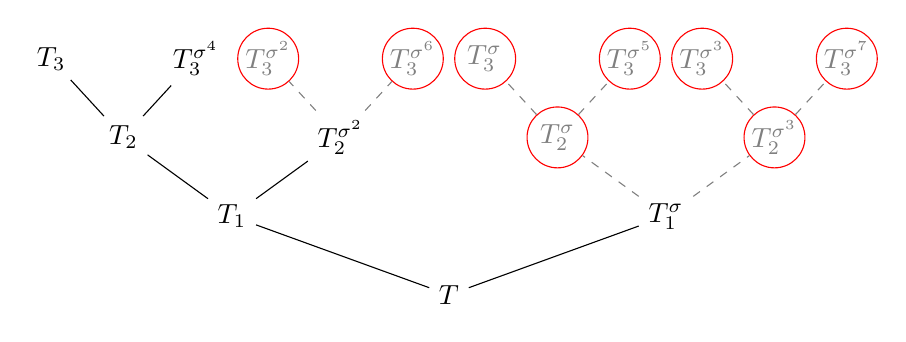
\begin{tikzpicture}
    \begin{scope}
      [level distance=1cm,
      level/.style={sibling distance=\textwidth/(2.2*#1)},
      nc/.style={gray,nodes={circle,draw=red,solid,inner sep=0pt,minimum size=22pt}}]
      \node{$T$}[grow'=up]
      child {node {$T_1$}
        child {node {$T_2$}
          child {node {$T_3$}}
          child {node {$T_3^{\sigma^4}$}}
        }
        child {node {$T_2^{\sigma^2}$}
          child[nc] foreach \l in {2,6} {node {$T_3^{\sigma^{\l}}$} edge from parent[dashed]}
        }
      }
      child {node {$T_1^\sigma$}
        child[nc] {node {$T_2^\sigma$} edge from parent[dashed]
          child[nc] foreach \l in {,5} {node {$T_3^{\sigma^{\l}}$} edge from parent[dashed]}
        }
        child[nc] {node {$T_2^{\sigma^3}$} edge from parent[dashed]
          child[nc] foreach \l in {3,7} {node {$T_3^{\sigma^{\l}}$} edge from parent[dashed]}
        }
      };
    \end{scope}
  \end{tikzpicture}
  
  \pdfmctwo{Circled nodes.}
  \caption{The subproduct tree of $T$, in the case of a tower of
    quadratic extensions. Any generator of $\Gal(\U_3/\U_0)$ can be
    taken as $\sigma$. We gray out and circle the nodes that the
    algorithm does not compute.}
  \label{fig:tree}
\end{figure}


Now the we have something like a subproduct tree for $T$, we proceed
as for interpolation. We compute recursively the polynomials in
$A_i\in\U_i[X]$ such that $A_i(x)=y$. We start from $A_k=y$. Suppose
$A_{i+1}$ is known, then we use the \titleref{th:chinese-remainder} to
obtain the polynomial $P\in\U_{i+1}[X]/T_i(X)$ such that
\begin{equation}
  \label{eq:crt}
  P \equiv A_{i+1}^\sigma \bmod T_{i+1}^\sigma
  \qquad\text{for any $\sigma\in\Gal(\U_{i+1}/\U_i)$.}
\end{equation}
It is clear that $P$ is invariant under $\Gal(\U_{i+1}/\U_i)$, hence
$P\in\U_i[X]/T_i(X)$ and by \eqref{eq:crt} it is evident that
$P(x)=A_{i+1}(x)=y$, thus $P=A_i$.

\pdfmctwo{Éric asked for the difference between Enge-Morain and this
  section. There is none in the algorithm, so I must at least say
  something about what is new in this section. Btw, the "Hecke
  representation" is just an instance of rational univariate
  representation.} We have thus succeeded in interpolating $A=A_0$,
without having to build the whole subproduct tree. A similar algorithm
was applied by Enge and Morain to the solution of equations by
radicals~\cite{enge+morain03}, although they did not recognize the
application to polynomial interpolation.

\begin{remark}
  Observe that, once the polynomials $T_i$ for $0\le i\le k$ are
  known, we have an efficient algorithm to evaluate polynomials in
  $g\in\U_0[X]$ at the point $x$: simply compute
  \begin{equation}
    \label{eq:191}
    \begin{aligned}
      g_0 &= g\bmod T_0\text{,}\\
      g_1 &= g_0\bmod T_1\text{,}\\
      \vdots\\
      g_k &= g_{k-1}\bmod T_k\text{,}\\
    \end{aligned}
  \end{equation}
  then $g_k=g(x)$. Transposing this algorithm gives a power projection
  algorithm that can be used in \titleref{alg:rur}. By the discussion in
  Section~\ref{sec:transp-eucl-divis}, the
  \index{transposed~modular~reduction}transpose of this algorithm
  amounts to iteratively extend a linearly recurring
  sequence. However, we do not use this method because it would not
  improve the overall complexity, as we shall show in the next
  section.
\end{remark}


\paragraph{Back to our problem}
It is easy to realize that, on inputs $x(P)$ and $x(P')$, the
algorithm we just gave computes $A^{(0)}$. In fact, $T^{(0)}$ is
the minimal polynomial of $x(P)$ over $\F_q$ and $A^{(0)}$ is the
unique polynomial in $\F_q[X]/T^{(0)}(X)$ that satisfies
\eqref{eq:affine-minimal}.

This can be viewed as decomposing the morphism $\iota$ of
Eq.~\eqref{eq:embed} as the chain of $\F_q$-linear isomorphisms
\begin{equation}
  \xymatrix{
    ^{\U_0[X_0]}/_{T_0(X_0)} \ar@{^{(}->}[r]^-{\iota_0} &
    \;\cdots\; \ar@{^{(}->}[r]^-{\iota_{k-1}} &
    ^{\U_k[X_k]}/_{T_k(X_k)} \ar@{^{(}->}[r]^-{\iota_k} &
    \U_k
  }
\end{equation}
defined by $\iota_k\circ\cdots\circ\iota_i(X_i) = x(P)$ for any $i$,
and then finding the preimage of $x(P')$ by inverting them one by
one.

Then, the Chinese remainder theorem we applied in \eqref{eq:crt}
amounts to invert $\iota_i$ by descending the lower path in the
diagram below
\begin{equation}
  \xymatrix{
    ^{\U_i[X_i]}/_{T_i(X_i)} \ar@{^{(}->}[r]^-{\iota_i} \ar@{^{(}->}[d]^{\varepsilon} &
    ^{\U_{i+1}[X_{i+1}]}/_{T_{i+1}(X_{i+1})} \\
    ^{\U_{i+1}[Y]}/_{T_i(Y)} \ar@{^{(}->>}[r]^-{\gamma} &
    \bigoplus_\sigma {}^{\U_{i+1}[Y_{j}]}/_{\left(T_{i+1}\right)^\sigma(Y_{j})} \ar@{->>}[u]_{\pi}
  }
\end{equation}
where $\varepsilon$ is the canonical injection extending
$\U_i\subset\U_{i+1}$, $\gamma$ is the Chinese remainder isomorphism
and $\pi$ is projection onto the first coordinate.

Some care must be taken when $x(P)$ does not generate $\U_k$, but only
a subfield of index $2$. This happens when $c\not\in\F_q[c^2]$, and in
this case $\iota_0$ is not a field isomorphism. It is not to
difficult, however, to handle this case, as one only needs to take a
subgroup of index $2$ of $\Gal(\U_1/\U_0)$, instead of the whole
group, in the interpolation algorithm given above.


\subsection{Complexity analysis}
\label{sec:C2-AS-FI:complexity}

In practice, the algorithms to compute $T^{(0)}$ and $A^{(0)}$ are
modified versions of the subproduct tree and the interpolation (see
Section~\ref{sec:chin-rema-algor}).

We set some notation. Let $i_0$ be the largest index such that
$\U_{i_0} = \U_1$ and let $\frac{p-1}{2r} = [\F_q[c^2]:\F_q]$.  Note
that all the $T^{(j)}$'s have degree $\frac{\euler(p^{k-i_0+1})}{2r}$.

We first compute the \emph{truncated} subproduct tree as in
Figure~\ref{fig:tree}. The product of Eq.~\eqref{eq:minprod} is
computed via a classic binary subproduct tree to keep the complexity
low.

\begin{algorithm}
  \caption{Truncated subproduct tree}
  \begin{algorithmic}[1]
    \REQUIRE $x(P)\wrt\U_k$.
    \ENSURE The subproduct tree.
    \STATE Let $T_k = (X - x(P))$;
    \FOR {$i=k-1$ \TO $0$}
    \FORALL {$\sigma \in \Gal(\U_{i+1}/\U_i)$}
    \STATE\label{alg:T:gal} compute $T_{i+1}^\sigma$  using \titleref{alg:iterfrobenius};
    \ENDFOR
    \STATE\label{alg:T:prod}  $T_i\la\prod_\sigma T_{i+1}^\sigma$ 
    via a binary \hyperref[sec:chin-rema-algor]{subproduct tree}.
    \STATE\label{alg:T:push} convert $T_i$  into an element of
    $\U_i[X]$ using \titleref{alg:push-down}.
    \ENDFOR
  \end{algorithmic}
\end{algorithm}

Recall that we denote by $\Lift(i)$ the cost of performing one lift-up
or push-down at the $i$-th level (see Theorem~\ref{theo:L}). For any
$i>i_0$, step~\ref{alg:T:gal} of is repeated $p$ times, each iteration
taking 
\[O\bigl(p^{k-i}\Lift(i-i_0)\bigr) \subset O\bigl(\Lift(k-i_0)\bigr)\]
by Theorem~\ref{th:b-ifrob}.  Step~\ref{alg:T:prod} takes
$O\bigl(\Mult(p^{k-i_0+1}d/r)\log p\bigr)$ using
Algorithm~\ref{alg:subprod} and step~\ref{alg:T:push} takes
\[O\bigl(p^{k-i+1}\Lift(i-i_0)\bigr) \subset
O\bigl(p\Lift(k-i_0)\bigr)\text{.}\]

For any $1\le i<i_0$, there is nothing to do because
$\U_{i+1}=\U_i$. Finally, when $i=0$ and $\U_1\ne\F_q$ the algorithm
is identical but step \ref{alg:T:gal} must be computed through a
generic Frobenius algorithm (using the algorithm of
Section~\ref{sec:modular-composition}, for example) and step
\ref{alg:T:push} must use the implementation of $F_q[c]$ to make the
conversion (for example, linear algebra). In this case
step~\ref{alg:T:gal} costs
$\Theta\bigl(\frac{p^{k-i_0}}{r}\ModComp(pd)\log d \bigr)$
by Eq.~\eqref{eq:204} and step \ref{alg:T:push} costs
$\Theta\bigl(p^{k-i_0}(pd)^2\bigr)$.

Now, we have $T_0$ at the root of the tree. We compute its derivative
$T_0'$ and we evaluate it at $x(P)$ by reducing modulo
$T_1,\ldots,T_k$. This costs strictly less than computing the
subproduct tree.  We finally do the interpolation of $A_0$.

\begin{algorithm}
  \caption{Truncated fast interpolation}
  \begin{algorithmic}[1]
    \REQUIRE $T_i\wrt\U_i[X]$ for $0\le i\le k$, $x(P')\wrt\U_k$, $T_0'(x(P))\wrt\U_k$.
    \ENSURE $A_0\wrt\U_0[X]$.
    \STATE\label{alg:A}  $P_k \la x(P')/T_0'(x(P))$;
    \FOR {$i = k-1$ \TO $0$}
    \FORALL {$\sigma \in \Gal(\U_{i+1}/\U_i)$}
    \STATE\label{alg:A:gal} compute $P_{i+1}^\sigma$ using \titleref{alg:iterfrobenius};
    \ENDFOR
    \STATE\label{alg:T:lift} convert $T_i$ into an element of $\U_{i+1}[X]$ using \titleref{alg:liftup}.
    \STATE\label{alg:A:CRA} $P_i\la \sum_{\sigma}P_{i+1}^\sigma T_i/T_{i+1}^\sigma$ using the binary subproduct tree computed previously;
    \STATE\label{alg:A:push} convert  $P_i$ into an element of
    $\U_i[X]$ using \titleref{alg:push-down}.
    \ENDFOR
    \STATE return $P_0$.
  \end{algorithmic}
\end{algorithm}

Step~\ref{alg:A} is just one inversion in $\U_k$, that is
$O(\Mult(p^{k-i_0}d/r)\log p^{k-i_0}d/r)$. Steps~\ref{alg:A:gal}
and~\ref{alg:A:push} are identical to steps~\ref{alg:T:gal}
and~\ref{alg:T:push} of the subproduct tree and step~\ref{alg:T:lift}
is also absorbed. Finally, step~\ref{alg:A:CRA} has the same
complexity as step~\ref{alg:T:prod} of the subproduct tree, using the
Algorithm~\ref{alg:interp}.

In conclusion, the total cost of computing the subproduct tree and the
interpolation is
\ifafourps
\begin{equation*}
  O\biggl(\bigl(k-i_0\bigr)p\Lift(k-i_0) + \Mult\left(\frac{p^{k-i_0+1}d}{r}\right)\log \frac{p^{k-i_0}d}{r} +
  \frac{p^{k-i_0}}{r}\bigl(\ModComp(pd)\log d + r(pd)^2\bigr)\biggr)
  \text{.}
\end{equation*}
\else
\begin{multline*}
  O\biggl(\bigl(k-i_0\bigr)p\Lift(k-i_0) + \Mult\left(\frac{p^{k-i_0+1}d}{r}\right)\log \frac{p^{k-i_0}d}{r} +\\
  \frac{p^{k-i_0}}{r}\bigl(\ModComp(pd)\log d + r(pd)^2\bigr)\biggr)
  \text{.}
\end{multline*}
\fi

\paragraph{The complete interpolation}
We compute all the $A^{(j)}$'s using this algorithm; there are
$p^{i_0-1}r$ of them. We then recombine them through a
\hyperref[sec:chin-rema-algor]{Chinese remainder algorithm} at a cost
of $O\bigl(\Mult(p^kd)\log p^kd\bigr)$. The total cost of the whole
interpolation phase is then
\begin{equation*}
  O\left(\bigl(k-i_0\bigr) p\Lift(k) + p^{k-1}\ModComp(pd)\log d +
    p^{k-1}r(pd)^2 + \Mult(p^kd)\log p^kd \right)\text{,}
\end{equation*}
that is
\begin{equation}
  \label{eq:interp}
  O\left(p\Lift(k)\log\left(\frac{\ell}{p^{i_0}}\right) + 
    \Mult(\ell d)\log\ell d +
    \frac{\ell}{p}\ModComp(pd)\log d +
    \ell (pd)^2
  \right)\text{.}
\end{equation}

Alternatively, once $A^{(0)}$ is known, one could compute the other
$A^{(j)}$'s using modular composition with the multiplication maps of
$E$ and $E'$ as suggested in~\cite{couveignes96}. However this
approach does not give a better asymptotic complexity because in the
worst case $A^{(0)}=A$. From a practical point of view, though,
Brent's and Kung's algorithm for modular
composition~\cite{brent+kung}, despite having a worse asymptotic
complexity, could perform faster for some set of parameters. We will
discuss this matter in Section~\ref{sec:C2-AS-FI-MC}.

If more than $\euler(p^k)/2$ points are needed, but less than
$\frac{p-1}{2}$, one can use the previous algorithm to interpolate
over the primitive $p^i$-torsion points for each $i=1,\ldots,k$. The
interpolating polynomials can then be recombined through a
\hyperref[sec:chin-rema-algor]{Chinese remainder algorithm} at a cost
of $O\bigl(\Mult(p^kd)\log p^k\bigr)$, which does not change the
overall complexity of \ctwoasfi{}.


Putting together the complexity estimates of \ctwoas{} and \ctwoasfi{}, we
have the following theorem.

\begin{theorem}
  \label{th:complexity}
  Assuming $\Mult(n) = n\log n\loglog n$, the algorithm \ctwoasfi{} has
  worst case complexity
  \ifafive
  \begin{multline*}
    \tildO_{p,d,\log\ell}
    \left(
      p^2d^3 +
      \ModComp(p)pd +
      (pd)^\omega\log^2\ell +
      p^3\ell^2 d\log^3\ell + \right.\\
      \left. p^2\ell^2 d^2+
      \left(\frac{\ell^2}{p} + p\right)\ModComp(pd)
    \right)
    \text{.}
  \end{multline*}
  \else
  \begin{equation*}
    \tildO_{p,d,\log\ell}
    \ifbfive\!\fi
    \left(
      \ifbfive\!\fi
      p^2d^3 +
      \ModComp(p)pd +
      (pd)^\omega\log^2\ell +
      p^3\ell^2 d\log^3\ell + 
      p^2\ell^2 d^2+
      \left(\ifbfive\!\fi\frac{\ell^2}{p} + p\ifbfive\!\fi\right)\ModComp(pd)
      \ifbfive\!\fi
    \right)
    \ifbfive\!\fi
    \text{.}
  \end{equation*}
  \fi
\end{theorem}



% Local Variables:
% mode:flyspell
% ispell-local-dictionary:"american"
% mode:TeX-PDF
% TeX-master: "../these"
% mode:reftex
% End:
%
% LocalWords:  Schreier Artin pseudotrace Frobenius bivariate Joux Sirvent FFT
% LocalWords:  Couveignes isogenies Schoof isogeny cryptosystems Lercier moduli
% LocalWords:  precomputation arithmetics polylogarithmic Karatsuba embeddings
% LocalWords:  irreducibility

\section{The algorithm \alg{C2-AS-FI-MC}}
\label{sec:C2-AS-FI-MC}

However asymptotically fast, the polynomial interpolation step is
quite expensive for reasonably sized data. Instead of repeating it
$\frac{\euler(p^k)}{2}$ times, one can use composition with the
Frobenius endomorphism $\frobisog_E$ in order to reduce the number of
interpolations in the final loop. We call this variant \ctwoasfimc{} (MC
for Modular Composition).

\subsection{The algorithm}
Suppose we have computed, by the algorithm of the previous Section,
the polynomial $T$ vanishing on the abscissas of $E[p^k]$ and an
interpolating polynomial $A_0\in\F_q[X]$ such that
\begin{equation*}
  A_0\bigl(x\bigl([n]P\bigr)\bigr) = x\bigl([n]P'\bigr)
  \quad\text{for any $n$.}
\end{equation*}
We view $A_0$ as a morphism of varieties (not necessarily an isogeny!)
from $E[p^k]$ to $E'[p^k]$.

The \hyperref[sec:curves-over-finite]{Frobenius automorphism}
$\frobisog_E$ acts on $E[p^k]$ permuting its points. We define
\begin{equation}
  \label{eq:183}
  A_1\eqdef A_0\circ\frobisog_E = \frobisog_{E'}\circ A_0
  \text{,}
\end{equation}
where the equality comes from the fact that $A_0$ is
$\F_q$-rational. Hence
\begin{equation*}
  A_1\circ[n](P) = [n]\circ\frobisog_{E'}(P')
  \quad\text{for any $n$.}
\end{equation*}
$A_1$ has no poles at $E[p^k]$, thus it is a polynomial map; and since
$\frobisog_{E'}(P')$ is a generator of $E'[p^k]$, $A_1$ is one of the
polynomials that the algorithm \ctwo{} tries to identify to an isogeny. By
iterating this construction we obtain $[\U_k:\F_q]/2$ different
polynomials $A_i$ for the algorithm \ctwo{} with only one interpolation.

To compute the $A_i$'s, we first compute $F\in\F_q[X]$
\begin{equation}
  \label{eq:frob}
  F(X) = X^q \bmod T(X)
  \text{,}
\end{equation}
then for any $1\le i<[\U_k:\F_q]/2$
\begin{equation}
  \label{eq:modcomp}
  A_i(X) = A_{i-1}(X)\circ F(X) \bmod T(X)\text{.}
\end{equation}

If $\frac{\euler(p^k)}{[\U_k:\F_q]} = p^{i_0-1}r$, we must compute
$p^{i_0-1}r$ polynomial interpolations and apply this algorithm to
each of them in order to deduce all the polynomials needed by \ctwo{}.


\subsection{Complexity analysis}
We compute \eqref{eq:frob} via square-and-multiply, this costs
$\Theta(d\Mult(p^kd)\log p)$ operations. Each application of
\eqref{eq:modcomp} is done via a
\hyperref[sec:modular-composition]{modular composition}, the cost is
thus $O(\ModComp(p^k))$ operations in $\F_q$, that is
$O(\ModComp(p^k)\Mult(d))$ operations in $\F_p$. Using the algorithm
of~\cite{kedlaya+umans08} for modular composition, the complexity of
\ctwoasfimc{} would not be essentially different from the one of
\ctwoasfi{}. However, in practice the fastest algorithm for modular
composition is~\cite{brent+kung}, and in particular the variant
in~\cite[Lemma~3]{kaltofen+shoup98}: these have worse asymptotic
complexity, but perform better on the instances we treat in
Section~\ref{sec:benchmarks}.

Notice that a similar approach could be used inside the polynomial
interpolation step (see Section \ref{sec:C2-AS-FI}) to deduce
$A_k^{(0)}$ from $A_0^{(0)}$ using modular composition with the
multiplication maps of $E$ and $E'$ as described in
\cite[$\S$2.3]{couveignes96}. This variant, though, has an even worse
complexity because of the cost of computing multiplication maps.




% Local Variables:
% mode:flyspell
% ispell-local-dictionary:"american"
% mode:TeX-PDF
% mode:reftex
% TeX-master: "../these"
% End:
%
% LocalWords:  Schreier Artin pseudotrace Frobenius bivariate Joux Sirvent FFT
% LocalWords:  Couveignes isogenies Schoof isogeny cryptosystems Lercier moduli
% LocalWords:  precomputation arithmetics polylogarithmic Karatsuba embeddings
% LocalWords:  irreducibility

\section{Smallest degree isogeny}
\label{sec:bounded}

We now present an extension to Couveignes algorithm that could be
useful in cryptographic application. It is well known that two curves
having the same number of points over a finite field are isogenous,
however this doesn't say anything on the degree of the isogeny
connecting them. Given two elliptic curves $E$ and $E'$ defined over
$\F_q$ and having the same number of points, we want to find the
smallest degree isogeny between them.

The simplest solution is to take any algorithm computing a fixed
degree isogeny and try all the degrees until an isogeny is found. If
$\ell$ is the degree of the smallest isogeny, this of course adds a
factor $\ell$ to the complexity of any polynomial time algorithm.

Couveignes' algorithm can be easily adapted to solve this problem at
no additional cost. We call this algorithm C2SD and we will only
discuss its most efficient variant C2SD-AS-FI.

Observe that, apart for the choice of $k$, the computation of $E[p^k]$
and the polynomial interpolation step do not depend at all on
$\ell$. The degree of the isogeny only comes into play in the last
part of the Cauchy interpolation, that is the rational function
reconstruction. We study more in detail this last step.


\paragraph{Rational Function Reconstruction}
Rational function reconstruction takes as input a degree $n$
polynomial $T$, a polynomial $A$ of degree less than $n$ and a target
degree $m\le n$ and outputs the unique rational function such that
\begin{equation*}
  A \equiv \frac{R}{V} \bmod T
\end{equation*}
and $\deg R < m$, $\deg V \le n-m$. This is done by computing a Bezout
relation $AV + TU = R$ with the expected degrees via an XGCD
algorithm. If a classical XGCD algorithm is used, one simply computes
all the lines
\begin{equation}
  \label{eq:XGCD}
  \begin{aligned}
    R_0 &= T, & U_0 &= 1, & V_0 &= 0,\\
    R_1 &= A, & U_1 &= 0, & V_1 &= 1,\\
    R_{i-1} &= Q_iR_i + R_{i+1}, & U_{i+1} &= U_{i-1}-Q_iU_i, & V_{i+1} &= V_{i-1}-Q_iV_i
  \end{aligned}
\end{equation}
and stops as soon as a remainder $R_{i+1}$ with $\deg R_{i+1}<m$ is
found. If a fast XGCD algorithm as \cite[Algo. 11.4]{vzGG} is used,
one directly aims at the two lines
\begin{equation}
  \label{eq:FastGCD}
  \begin{aligned}
    R_{h-2} &= Q_{h-1}R_{j-1} + R_h\\
    R_{h-1} &= Q_hR_h + R_{h+1}
  \end{aligned}
\end{equation}
such that $\deg R_{h+1} < m \le \deg R_h$ without computing the
intermediate lines.

When looking for an $\ell$-isogeny, one simply sets
$m=\ell+1$. Observe that if the algorithm doesn't return a rational
fraction $\frac{R}{V}$ with $\deg R = \ell$ and $\deg V = \ell -1 $,
then no such fraction congruent to $A$ modulo $T$ exists.

If $\ell$ is not \emph{a priori} known, we can still use the fact that
a separable isogeny with cyclic kernel must have $\deg R = \deg V +
1$. In fact if we suppose $R = R_i$ and $V = V_i$, then
\begin{align*}
  \deg T &= \deg V_{i+1} + \deg R_i,\\
  \deg R_i - \deg V_i &= \deg R_{i-1} - \deg V_{i+1}
\end{align*}
implies
\begin{equation*}
  \deg T + 1 = \deg R_{i-1} + \deg R_i  
  \;\text{.}
\end{equation*}
Hence, if $A$ is congruent to an $\ell$-isogeny with $\ell =
\left\lfloor\frac{\deg T}{2}\right\rfloor - t$ for some $t\ge0$, then
\begin{equation}
  \label{eq:degseq}
  \deg R_{i-1} =
  \left\lceil\frac{\deg T}{2}\right\rceil + t + 1 >
  \left\lfloor\frac{\deg T}{2}\right\rfloor - t = \deg R_i
  \;\text{.}
\end{equation}
Thus we can recover any isogeny having degree less than
$\left\lfloor\frac{\deg T}{2}\right\rfloor$ using either a classical
or a fast XGCD algorithm setting $m = \left\lceil\frac{\deg
    T}{2}\right\rceil + 1$.


\paragraph{Recognising an isogeny}
Once we have a rational fraction with the required degree, we have to
test if it really is an isogeny. In order to understand how often we
have to make this test, we introduce some more terminology. Let $n_i =
\deg R_i$, we call $(n_0,\ldots,n_r)$ the \emph{degree sequence} of
$A$ and $T$; a degree sequence is said \emph{normal} if $n_i = n_{i+1}
+ 1$ for any $i$.

\begin{proposition}
  \label{th:normseq}
  Let $f,g\in\F_q[X]$ be uniformly chosen random polynomials of
  respective degrees $n_0>n_1>0$ and let $(n_0, n_1, \ldots, n_r)$ be
  their degree sequence. For $0\le i < n_1$ define the binary random
  variables $X_i = 1 \Leftrightarrow i\in(n_0,n_1,\ldots,n_r)$, then
  the $X_i$ are independent random variables and $\mathrm{Prob}(X_i=0) =
  \frac{1}{q}$.
\end{proposition}
\begin{proof}
  Pairs of polynomials $f,g$ are in bijection with the GCD-sequence
  $(R_r, Q_r, \ldots, Q_1)$ constituted by their GCD and the quotients
  of the GCD algorithm. To each such sequence is associated a degree
  sequence
  \begin{equation*}
    (n_0,n_1,\ldots,n_r) =
    \left(\deg R_r + \sum_{i=1}^r\deg Q_i, \ldots, \deg R_r + \sum_{i=1}^1\deg Q_i, \deg R_r\right)
    \;\text{,} 
  \end{equation*}
  thus for any given degree sequence there are
  \begin{equation*}
    (q-1)q^{n_0-n_1}\cdot(q-1)q^{n_1-n_2}\cdot\cdots\cdot(q-1)q^{n_r} =
    (q-1)^{r+1}q^{n_0}
  \end{equation*}
  GCD-sequences.
 
  Let $I$ and $O$ be two disjoints subsets of $\{X_i\}$, the number of
  GCD-sequences such that $X\in I \Rightarrow X=1$ and $X\in O
  \Rightarrow X=0$,
  \begin{equation*}
     \sum_{s=0}^{n_1-\card{I}-\card{O}}\binom{n_1-\card{I}-\card{O}}{s}(q-1)^{s+2+\card{I}}q^{n_0} =
    (q-1)^{2+\card{I}}q^{n_0}q^{n_1-\card{I}-\card{O}}
    \;\text{.}
  \end{equation*}
  There are $(q-1)^2q^{n_0}q^{n_1}$ pairs of polynomials of degrees
  $n_0,n_1$, thus
  \begin{equation}
   \label{th:normseq:prob}
    \mathrm{Prob}\bigl(\{X = 1 \mid X\in I\},
    \{X=0\mid X\in O\}\bigr) = \left(\frac{q-1}{q}\right)^{\card{I}}\left(\frac{1}{q}\right)^{\card{O}}
    \;\text{.}
  \end{equation}
  The claim follows.
\end{proof}

Degree sequences associated to isogenies are in general not normal, in
fact if $\ell\le\left\lfloor\frac{\deg T}{2}\right\rfloor-t$, equation
\eqref{eq:degseq} shows that there must be at least a gap of degree
$2c$ in the degree sequence. Heuristically, we can expect that if the
polynomial $A$ doesn't correspond to an isogeny, then $A$ and $T$ act
like random polynomials, thus, by the proposition above, the
probability that $A$ looks like an isogeny of degree
$\ell\le\left\lfloor\frac{\deg T}{2}\right\rfloor-t$ is less than $\frac{1}{q^{2t}}$.

Therefore, by choosing an appropriate $t\in O(\log_q p^k)$, C2SD can
find any isogeny of degree less than $\frac{p^k-1}{4}-t$ at the same
cost of one run of C2. Also notice that C2SD is not restricted to
isogenies of degree prime to $p$ as it was already mentioned in
Section \ref{sec:C2:non-prime}.

No other method for computing isogenies is known to have a similar
generalisation, this makes C2SD-AS-FI interesting for practical
applications.




% Local Variables:
% mode:flyspell
% ispell-local-dictionary:"british"
% mode:TeX-PDF
% TeX-master: "ec-isogeny"
% End:
%
% LocalWords:  Schreier Artin pseudotrace frobenius bivariate Joux Sirvent FFT
% LocalWords:  Couveignes isogenies Schoof isogeny cryptosystems Lercier
% LocalWords:  precomputation arithmetics polylogarithmic Karatsuba precomputes
% LocalWords:  endomorphisms  isogenous


\chapter{Experimental results}
In this chapter we describe the implementations we made of the
algorithms of the previous chapter and some experimental results.

\section{Implementation of Couveignes' algorithm}
\label{sec:implementation}

We implemented C2-AS-FI-MC as \texttt{C++} programs using the
libraries \texttt{NTL}~\cite{shoup2003ntl} for finite field
arithmetics, \texttt{gf2x}~\cite{gf2x} for fast arithmetics in
characteristic $2$ and \texttt{FAAST} (see
Section~\ref{sec:artin-benchmarks}) for fast arithmetics in
Artin-Schreier towers.  We also have a Magma~\cite{MAGMA} prototype of
the same algorithm, not making use of the fast algorithms of
Chapter~\ref{cha:artin-schr-towers}.  This section mainly deals with
some tricks we implemented in order to speed up the computation.

\subsection{Building \texorpdfstring{$E[p^k]$}{E[pk]} and \texorpdfstring{$E'[p^k]$}{E[pk]}}
\label{sec:impl:torsion}

\paragraph{$p$-Torsion}
For $p\ne2$, C2 and its variants require to build the extension
$\F_q[c]$ where $c$ is a $(p-1)$-th root of $H_E$. In order to deal with
the lowest possible extension degree, it is a good idea to modify the
curve so that $[\F_q[c]:\F_q]$ is the smallest possible.

$[\F_q[c]:\F_q]$ is invariant under isomorphism, but taking a twist
can save us a quadratic extension. Let $u=c^{-2}$, the curve
\begin{equation*}
  \bar{E} : y^2 = x^3 + a_2ux^2 + a_4u^2x + a_6u^3
\end{equation*}
is defined over $\F_q[c^2]$ and is isomorphic to $E$ over $\F_q[c]$
via $(x,y)\mapsto(\sqrt{u}^2x,\sqrt{u}^3y)$. Its Hasse invariant is
$H_{\bar{E}} = (u)^{\frac{p-1}{2}}H_E = 1$, thus its $p$-torsion
points are defined over $\F_q[c^2]$.

In order to compute the $p^k$-torsion points of $E$ we build
$\F_q[c^2]$, we compute $\bar{P}$ a $p^k$-torsion points of $\bar{E}$
using $p$-descent, then we invert the isomorphism to compute the
abscissa of $P\in E[p^k]$. Since the Cauchy interpolation only needs
the abscissas of $E[p^k]$, this is enough to complete the
algorithm. Scalar multiples of $P$ can be computed without knowledge
of $y(P)$ using \hyperref[rk:montgomery]{Montgomery formulas}.

\pdfmargincomment{"Kummer surface" -> "Kummer variety".}  Remark that
for $p=2$ we use the same construction in an implicit way since we do
a $p$-descent on the Kummer variety.


\paragraph{$p^k$-Torsion points}
For $p\ne2$ we use Voloch's $p$-descent to compute the $p^k$-torsion
points iteratively as described in Section \ref{sec:C2}. To factor the
Artin-Schreier polynomial \eqref{th:voloch:cover}, we use the
algorithms from Section~\ref{sec:couveignes-algorithm} implemented in
\texttt{FAAST}.

To solve system \eqref{th:voloch:isom} we first compute
\begin{equation*}
  V(x,y) = \left(\frac{g(x)}{h^2(x)}, 
    sy\left(\frac{g(x)}{h^2(x)}\right)'\right)
\end{equation*}
through \hyperref[sec:velu-formulas]{Vélu formulas}.\footnote{Vélu
  formulas compute this isogeny up to an indeterminacy on the sign of
  the ordinate, the actual value of $s$ must be determined by
  composing $V$ with $\frobisog$ and verifying that it corresponds to
  $[p]$ by trying some random points.} Recall that we work on a curve
having Hasse invariant $1$, system \eqref{th:voloch:isom} can then be
rewritten
\begin{equation*}
  \left\{
    \begin{aligned}
      \tilde{x}(P) &= \frac{g(x)}{h^2(x)}\\
      \tilde{y}(P) &= sy\left(\frac{g(x)}{h^2(x)}\right)'\\
      \tilde{z}(P) &= -2y\frac{h'(x)}{h(x)}
    \end{aligned}
  \right.
\end{equation*}
where $P$ is the point on the cover $C$ that we want to pull back
($\tilde{x}(P)$, $\tilde{y}(P)$ and $\tilde{z}(P)$ are just its
coordinates). After some substitutions this is equivalent to
\begin{equation*}
  \left\{
    \begin{aligned}
      \tilde{x}(P)h^2(x) - g(x) &= 0\\
      \left(\tilde{x}(P)h^2(x) - g(x) - \frac{\tilde{y}(P)}{s\tilde{x}(P)}h^2(x)\right)' &= 0
    \end{aligned}
  \right.
\end{equation*}
Then a solution in $x$ to this system is given by the GCD of the two
equations. Remark that proposition \ref{th:voloch} ensures there is
one unique solution. These formulas are slightly more efficient than
the ones in \cite[$\S$6.2]{lercier-algorithmique}.

For $p=2$ we use the library \texttt{FAAST} (for solving
Artin-Schreier equations) on top of \texttt{gf2x} (for better
performance). There is nothing special to remark about the
$2$-descent.


\subsection{Cauchy interpolation and loop}
\label{sec:impl:cauchy}
The polynomial interpolation step is done as described in Section
\ref{sec:C2-AS-FI}. As a result of this implementation, the polynomial
interpolation algorithm was added to the library \texttt{FAAST}.

The rational fraction reconstruction is implemented using a fast XGCD
algorithm on top of \texttt{NTL} and \texttt{gf2x}. This algorithm was
added to \texttt{FAAST} too.

The loop uses modular composition as in Section~\ref{sec:C2-AS-FI-MC}
in order to minimise the number of interpolations. The timings in the
next section clearly show that this non-asymptotically-optimal variant
performs much faster in practice.

To check that the rational fractions are isogenies we test their
degrees, that their denominator is a square and that they act as group
morphisms on a fixed number of random points. All these checks take a
negligible amount of time compared to the rest of the algorithm.


\subsection{Parallelisation of the loop}
\label{parallel}

The most expensive step of C2-AS-FI-MC, in theory as well as in
practice, is the final loop over the points of $E'[p^k]$. Fortunately,
this phase is very easy to parallelise with very little overhead.

Let $n$ be the number of processors we wish to parallelise on, suppose
that $[\U_k:\F_q]$ is maximal, then we make only one interpolation
followed by $\euler(p^k)/2$ modular compositions.\footnote{If
  $[\U_k:\F_q]$ is not maximal, the parallelisation is
  straightforward: we simply send one interpolation to each processor
  in turn.} We set $m=\left\lfloor\frac{\euler(p^k)}{2n}\right\rfloor$
and we compute the action of $\frobisog^{m}$ on $E[p^k]$ as in
Section~\ref{sec:C2-AS-FI-MC}:
\begin{equation*}
  F^{(m)}(X) = F(X) \circ \cdots \circ F(X) \bmod T(X)
  \;\text{,}
\end{equation*}
this can be done with $\Theta(\log m)$ modular compositions via a
binary square-and-multiply approach as in
Section~\ref{sec:modular-composition}.

Then we compute the $n$ polynomials
\begin{equation*}
  A_{mi}(X) = A_{m(i-1)}(X) \circ F^{(m)}(X) \bmod T(X)
\end{equation*}
and distribute them to the $n$ processors so that they each work on a
separate slice of the $A_i$'s. The only overhead is $\Theta(\log
(\ell/n))$ modular compositions with coefficients in $\F_q$, this is
acceptable in most cases.

\section{Implementation of C2-UD}
\label{sec:implementation-c2-ud}
We modified our \texttt{C++} implementation of C2-AS-FI-MC to obtain
two variants of C2-UD.

The first one takes an integer $k$ and looks for all isogenies of
degree $p^c\ell$ with $\ell$ prime to $p$, $\ell<\euler(p^k)/4$
and $c$ arbitrary. This is done by slightly modifying the modular
composition step of Section~\ref{sec:C2-AS-FI-MC}. Suppose we know an
interpolating polynomial $A_0$, that we view as a morphisms $E[p^k]\ra
E'[p^k]$ such that
\begin{equation}
  \label{eq:184}
  A_0\circ[n](P) = [n](P')
  \quad\text{for any $n$.}
\end{equation}
Then we compose with the Frobenius isogeny $\frobisog$
\begin{equation}
  \label{eq:185}
  A_1 \eqdef \frobisog\circ A_0:E[p^k]\ra {E'}^{(p)}[p^k]
  \text{,}
\end{equation}
where ${E'}^{(p)}$ is the curve
\begin{equation}
  \label{eq:186}
  E^{(p)}\;:\; y^2 = x^3+{a'}^px + {b}'^p
  \text{.}
\end{equation}
So $A_1$ is one of the polynomials that Couveignes algorithm computes
when looking for an isogeny between $E$ and ${E'}^{(p)}$. If $q=p^d$,
iterating $d$ times this construction, we fall back on $E'$, as we
would have if we had directly applied the
\hyperref[sec:curves-over-finite]{Frobenius automorphism} as in
Section~\ref{sec:C2-AS-FI-MC}. Thus, paying an additional factor of
$\log_p q$, we can compute any isogeny of degree $p^c\ell$ with
arbitrary $c$ and $\ell$ bounded as before.

When $\log_pq$ is large, the previous variant becomes unpractical. We
implemented a second variant using the algorithm described in
Section~\ref{sec:C2:non-prime}, this allows to compute any isogeny of
degree $\ell\le\euler(p^k)/4$, even if $p$ divides $\ell$. The
asymptotic cost of this variant is the same as one run of C2-AS-FI-MC,
because the search for $\ell$ prime to $p$ dominates.



\section{Implementation of Lercier-Sirvent}
We implemented a Magma prototype of \hyperref[alg:bmss]{\alg{BMSS}}
and \hyperref[alg:le-si]{\alg{Lercier-Sirvent}}. In both cases we did
not take Remark~\ref{rk:bmss} into account, and only implemented the
variant using rational fraction reconstruction. We used Magma native
support for $p$-adics to construct the field $\Q_q$.

Both implementations differ from the description we gave in
Sections~\ref{sec:bmss} and~\ref{sec:lercier-sirvent} in that they
only take the degree $\ell$ and the equation of $E$ as input, and
compute an $\F_q$-isogenous curve, if it exists, by factoring the
modular polynomial in $\F_q[X]$.

Instead of the classical modular polynomials $\Phi_\ell$ we used
Atkin's canonical polynomials $\Modpol^c_\ell$ since they have smaller
coefficients and degree; this does not change the other steps of the
algorithm. 

The modular polynomials were not computed on the fly as suggested in
Section~\ref{sec:lercier-sirvent}, instead they were taken from the
tables precomputed in Magma. This implies that the implementation has
an asymptotic complexity cubic in $\ell$, however we will see that
even this implementation behaves well in practice.


% Local Variables:
% mode:flyspell
% ispell-local-dictionary:"american"
% mode:TeX-PDF
% TeX-master: "../these"
% mode:reftex
% End:
%
% LocalWords:  Schreier Artin pseudotrace Frobenius bivariate Joux Sirvent FFT
% LocalWords:  Couveignes isogenies Schoof isogeny cryptosystems Lercier Hasse
% LocalWords:  precomputation arithmetics polylogarithmic Karatsuba precomputes
% LocalWords:  endomorphisms 

\section{Benchmarks}
\label{sec:benchmarks}
We ran various experiments to compare the different variants of the
algorithm \ctwo{} between themselves and to \titleref{alg:le-si}. All
the experiments were run on four dual-core Intel Xeon E5520 (2.26GHz),
using the parallelized version of the algorithm in some cases. Magma
2.16 was used to run Magma experiments.

\paragraph{Magma vs. \texttt{FAAST}}
\label{sec:magma-vs.-textttf}
The first set of experiments was run to evaluate the benefits of using
the algorithms of Chapter~\ref{cha:artin-schr-towers}. We selected
pairs of isogenous curves over $\F_{2^{101}}$ such that the height of
the tower is maximal (observe that this is always the case for
cryptographic curves).  We compared the Magma prototype to the
\texttt{FAAST}-based implementation of \ctwoasfimc{} using the
\texttt{zz\_p} and \texttt{GF2} data types (see
Section~\ref{sec:artin-benchmarks}).

\begin{figure}
  \centering
  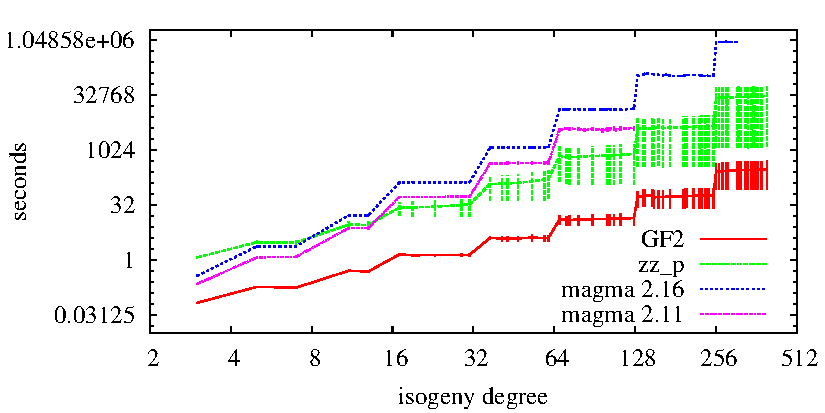
\includegraphics[width=0.9\textwidth]{isogeny/p2}
  \caption{Comparative timings for different implementations of \ctwoasfimc{} with curves defined over $\F_{2^{101}}$. Plot in logarithmic scale.}
  \label{fig:2-101}
\end{figure}

The results are in figure~\ref{fig:2-101}: we plot a line for the
average running time of the algorithm and bars around it for minimum
and maximum execution times of the final loop. Besides the dramatic
speedup obtained by using the ad-hoc type \texttt{GF2}, the
algorithmic improvements of \texttt{FAAST} over Magma are evident as
even \texttt{zz\_p} is one order of magnitude faster.

\begin{table}
  \centering
  \begin{tabular}{r r r r r r r r}
    \hline
    $\ell$ & $E[p^k]$ & $E'[p^k]$ & FI & RFR & MC & Avg tries & Avg loop time\\
    \hline
    31  &  0.3529 &  0.3529 & 0.3569 & 0.00125 & 0.00055 &  32 &   0.058\\
    61  &  0.9848 &  0.9848 & 0.8268 & 0.00343 & 0.00228 &  64 &   0.365\\
    127 &  2.6636 &  2.6626 & 1.8927 & 0.01090 & 0.00872 & 128 &   2.511\\
    251 &  6.9809 &  6.9779 & 4.2833 & 0.03092 & 0.03494 & 256 &  16.860\\
    397 & 18.1052 & 18.0952 & 9.7385 & 0.07325 & 0.14117 & 512 & 109.783\\
  \end{tabular}
  \caption{Comparative timings for the phases of \ctwoasfimc{} for curves over $\F_{2^{101}}$.}
  \label{tab:C2}
\end{table}

Table~\ref{tab:C2} shows detailed timings for each phase of
\ctwoasfimc{}. The column FI reports the time for one interpolation, the
column MC the time for one modular composition; comparing these two
columns the gain from passing from \ctwoasfi{} to \ctwoasfimc{} is
evident. Columns RFR (rational fraction reconstruction) and MC
constitute the Cauchy interpolation step that is repeated in the final
loop. The last column reports the average time spent in the loop: it
is by far the most expensive phase and this justifies the attention we
paid to FI and MC; only on some huge examples we approached the
crosspoint between these two algorithms.


\paragraph{\ctwoud{}}
\label{sec:c2-ud}
Next we ran experiments on \ctwoud{}. The first observation was that the
heuristic argument --on the probability that a degree sequence not
associated to an isogeny is not normal-- is well verified in practice:
except for a degree $2$ symmetry verified in characteristic $2$,
polynomials not associated to an isogeny very rarely gave a degree
sequence with a gap around the middle.

\pdfmcone{Added some blabla on Teske's cryptosystem.}
Looking for isogenies of unknown degree may be of some cryptographic
significance. For example, Teske's trapdoor cryptosystem selects a
binary field of composite degree ($\F_{2^{7\cdot 23}}$, in the
proposal) and chooses an elliptic curve $E$ vulnerable to the GHS
attack~\cite{gaudry+hess+smart02}. Then hides $E$ by taking a random
path of isogenies of small degrees landing on a curve $E'$ not
vulnerable to GHS, and uses $E'$ as public key. The security of the
cryptosystem comes from the assumption that it is infeasible to find a
GHS-vulnerable curve isogenous to $E'$, without the knowledge of the
isogeny path. 

The \emph{trapdoor} of the cryptosystem is the curve $E$: it is given
to a trusted authority so that --using an isogeny path from $E'$ to
$E$ and a GHS attack-- it has the power of deciphering messages at a
relatively high computational cost. This feature rests on the
assumption that it is feasible, but relatively hard, to compute any
isogeny path from $E$ to $E'$.

In this context, it may be interesting to verify that $E$ and $E'$ are
not related by an isogeny of too low degree.
From~\cite[Appendix~A]{teske06}, we took the two curves defined over
$F_{2^{161}}=\F_2[z]/(z^{161}+z^{18}+1)$ of $j$ invariants:

$1/j = z^{152} + z^{143} + z^{139} + z^{136} + z^{135} + z^{133} +
z^{130} + z^{125} + z^{124} + z^{122} + z^{120} + z^{119} + z^{118} +
z^{117} + z^{116} + z^{114} + z^{113} + z^{112} + z^{110} + z^{109} +
z^{106} + z^{105} + z^{103} + z^{102} + z^{101} + z^{99} + z^{97} +
z^{96} + z^{92} + z^{91} + z^{88} + z^{87} + z^{86} + z^{85} + z^{81}
+ z^{78} + z^{77} + z^{76} + z^{75} + z^{73} + z^{71} + z^{69} +
z^{68} + z^{67} + z^{66} + z^{63} + z^{59} + z^{58} + z^{53} + z^{51}
+ z^{50} + z^{49} + z^{48} + z^{46} + z^{45} + z^{44} + z^{42} +
z^{38} + z^{34} + z^{3} + z^{32} + z^{31} + z^{29} + z^{27} + z^{26} +
z^{24} + z^{23} + z^{22} + z^{21} + z^{20} + z^{19} + z^{18} + z^{17}
+ z^{16} + z^{15} + z^{14} + z^{13} + z^{12} + z^{10} + z^{7} + z^{6}
+ z^{4} + z^{3} + z^{2}$,

$1/j'=z^{160} + z^{156} + z^{155} + z^{153} +z^{152} +z^{151} +z^{150}
+z^{149} +z^{148} +z^{147} +z^{146} +z^{145} +z^{143} +z^{142}
+z^{141} +z^{130} +z^{129} + z^{127} + z^{126} + z^{125} + z^{124} +
z^{123} + z^{120} + z^{118} + z^{112} + z^{109} + z^{104} + z^{103} +
z^{102} + z^{101} + z^{99} + z^{98} +z^{97} +z^{96} +z^{93} +z^{92}
+z^{91} +z^{90} +z^{88} +z^{85} +z^{83} +z^{77} +z^{74} +z^{70}
+z^{68} +z^{65} +z^{64} +z^{63} + z^{62} + z^{61} + z^{60} + z^{58} +
z^{57} + z^{55} + z^{50} + z^{48} + z^{45} + z^{41} + z^{38} + z^{37}
+ z^{36} + z^{33} + z^{31} + z^{30} + z^{27} +z^{26} +z^{24} +z^{23}
+z^{22} +z^{21} +z^{20} +z^{19} +z^{17} +z^{16} +z^{14} +z^{13}
+z^{10} +z^{8} +z^{7} +z^{4} +z^{3} +z$.

We ran our two variants of \ctwoud{} on the two curves to certify the
conjectured property that no unexpected isogeny of low degree exists
between the two curves.

In 258 cpu-hours we were able to prove that no isogeny of degree
$p^c\ell$ for $\ell<2^{11}$ and $c$ arbitrary exists between the two
curves; in 694 cpu-hours we were able to prove that no isogeny of
degree less than $2^{13}$ exists either. We stress the fact that,
albeit of little interest, this computation would have been impossible
without the (surprising) discovery of \ctwoud{}.


\paragraph{Couveignes vs. Lercier-Sirvent}
Finally, we ran experiments on
\titleref{alg:le-si}. 
Table~\ref{tab:ls} shows
timings for the different phases of the algorithm for some isogeny
degrees. The first column is the time spent to find a root of
$\Modpol_\ell(X,j_E)$ in $\F_q$, the second column summarizes the time
spent to lift this root in $\Q_q$ and apply Elkies'
formulas. DiffSolve is the time spent solving the differential
equation, it is clearly the most expensive phase, although not the
most important asymptotically. RFR is the time for rational fraction
reconstruction, its rapid growth is justified by the fact that we
implemented it on top of a quadratic XGCD algorithm.

\begin{table}
  \pdfmcthree{This table has changed.}
  \centering
  \begin{tabular}{r r r r}
    \hline
    $\ell$ & Lift & DiffSolve & RFR\\
    \hline
    31  &   0.570 &   14.830 & 0.010\\
    103 &   5.160 &  274.550 & 0.250\\
    149 &  12.510 &  815.320 & 0.590\\
    239 &  21.420 & 1470.240 & 1.950\\
    331 & 113.500 & 4204.610 & 4.890\\
    389 & 147.340 & 5166.730 & 7.360\\
  \end{tabular}
  \caption{Comparative timings for the phases of \titleref{alg:le-si} 
    for curves over $\F_{3^{64}}$.}
  \label{tab:ls}
\end{table}


\begin{figure}
  \centering
  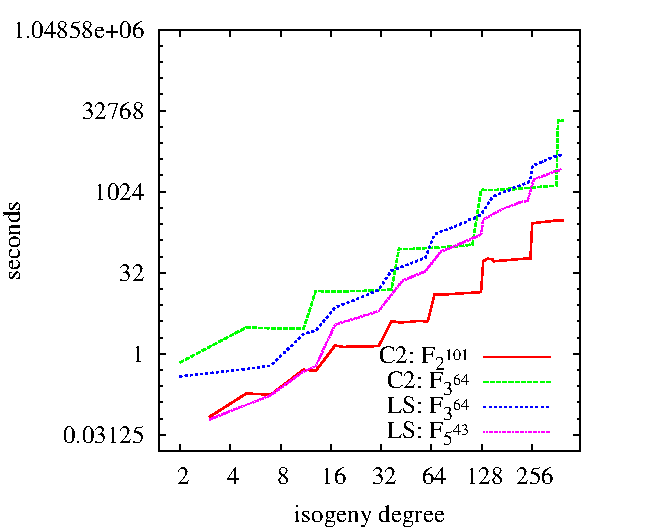
\includegraphics[height=0.45\textwidth]{isogeny/C2-LS}
  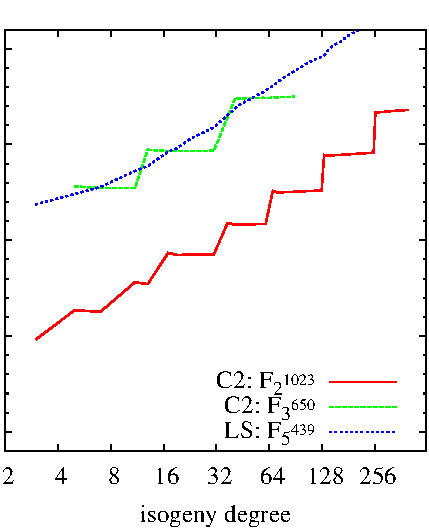
\includegraphics[height=0.45\textwidth]{isogeny/C2-LS2}
  \caption{Comparative timings for \ctwoasfimc{} (C2) and
    \titleref{alg:le-si} (LS) over different curves. Plot in
    logarithmic scale.}
  \label{fig:comp}
\end{figure}

We also compared the running times of \ctwoasfimc{} and
\titleref{alg:le-si} over curves of half the cryptographic size in
figure~\ref{fig:comp} (left) and five times the cryptographic size in
figure~\ref{fig:comp} (right). We only plot average times for \ctwo{},
in characteristic $2$ we only plot the timings for \texttt{GF2}. From
the plot it is clear that \ctwoasfimc{} only performs better than
\titleref{alg:le-si} for $p=2$, but in this case Lercier's
algorithm~\cite{lercier96} is much faster.  Contradicting theory, the
asymptotic behavior of \titleref{alg:le-si} looks worse than the one
of \ctwoasfimc{}; however comparing a Magma prototype to our highly
optimized implementation of \ctwoasfimc{} is somewhat unfair.

Furthermore, it is unlikely that \ctwoasfimc{} could be practical for
any $p>3$ because of its high dependence on $p$, while
\titleref{alg:le-si} scales pretty well with the characteristic as
shown in figure~\ref{fig:LSp}.

Considering that the asymptotic dependency of Couveignes' algorithm in
$\log q$ and in $p$ is worse than the one of \titleref{alg:le-si}
(compare Eq.~\eqref{eq:interp} to
Proposition~\ref{th:lercier-sirvent}), there are very few regions
where Couveignes' algorithm stays of practical or theoretical
interest.

\pdfmcone{People don't like pessimism.}  Ironically, the
techniques presented in this document were developed in view of an
efficient implementation of Couveignes' algorithm, but, for the
moment, their only practical application seems to be \ctwoud{}. Our hope
is that other interesting applications may be found in the future.

\begin{figure}
  \centering
  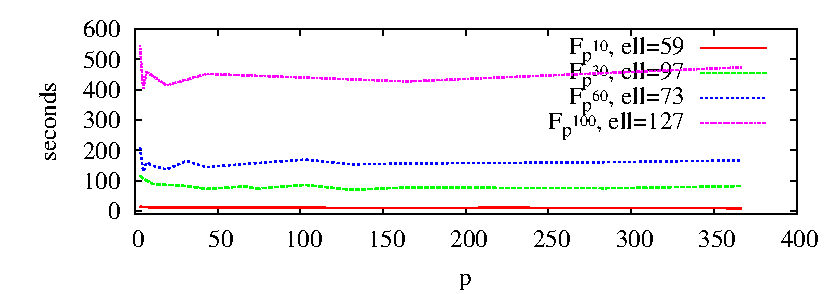
\includegraphics[width=0.9\textwidth]{isogeny/LSp}
  \caption{Timings for \titleref{alg:le-si} for different fields. We
    increase $p$ while keeping constant $d$ and the isogeny degree.}
  \label{fig:LSp}
\end{figure}


% Local Variables:
% mode:flyspell
% ispell-local-dictionary:"american"
% TeX-master: "../these"
% mode: TeX-PDF
% mode:reftex
% End:
%
% LocalWords:  Schreier Artin pseudotrace Frobenius bivariate Joux Sirvent FFT
% LocalWords:  Couveignes isogenies Schoof isogeny cryptosystems Lercier
% LocalWords:  precomputation arithmetics polylogarithmic Karatsuba precomputes
% LocalWords:  endomorphisms  isogenous



% Local Variables:
% mode:flyspell
% ispell-local-dictionary:"american"
% mode:TeX-PDF
% mode:reftex
% TeX-master: "../these"
% End:
%

